% Manual de usuario
% Modificado por Crisostomo Barajas a partir del manual creado por Emmanuel Martinez
% Julio 2022

\documentclass[12pt,twoside,letter]{ol-softwaremanual}
\usepackage{float}
\usepackage[utf8]{inputenc}
\usepackage[a4paper,width=160mm,top=25mm,bottom=25mm]{geometry}
\usepackage[lining,tabular]{fbb} % so math uses tabular lining figures
\usepackage{graphicx}
\usepackage{enumitem}
\setlist{leftmargin=*}
\usepackage{listings}
\lstset{basicstyle=\ttfamily,frame=single,xleftmargin=3em,xrightmargin=3em}
\usepackage[os=win]{menukeys}
\renewmenumacro{\keys}[+]{shadowedroundedkeys}
\usepackage{framed}
\usepackage{etoolbox}
\AtBeginEnvironment{leftbar}{\sffamily\small}
\usepackage{array,lipsum}
\newenvironment{fulltable}[1][H]
 {\begin{table}[#1]%
  \hspace*{-\leftmarginwidth}%
  \begin{minipage}{\fullwidth}}
 {\end{minipage}\end{table}}
\usetikzlibrary{chains,arrows,shapes,positioning}
\usepackage{hyperref}
\graphicspath{{figures/}} %Setting the graphicspath
\renewcommand\abstractname{Introduction}

\usepackage[spanish]{babel}

\usepackage{multicol}

\usepackage{caption}
\usepackage[rightcaption]{sidecap}
\usepackage{subcaption}
\usepackage{wrapfig}
\usepackage{pifont}
\usepackage{fontawesome}

\usepackage{amsmath}
\usepackage{amssymb}

\usepackage{fancyhdr}

\pagestyle{fancy}
\fancyhf{}
\fancyhead[LE,RO]{{\footnotesize HDSP - UIS}}
\fancyhead[RE,LO]{{\footnotesize ReDs - Ejemplos de Uso}}
\fancyfoot[CE,CO]{\thepage}
%\fancyfoot[LE,RO]{\thepage}

\definecolor{ClearPurple}{RGB}{136, 0, 255}

\usepackage{tikz}
\newcommand*\circled[1]{\tikz[baseline=(char.base)]{
            \node[shape=circle,draw,inner sep=2pt] (char) {#1};}}

\newenvironment{Figure}
  {\par\medskip\noindent\minipage{\linewidth}}
  {\endminipage\par\medskip}
  
%\setlength{\parskip}{2em}
\setlength{\parskip}{6pt}%
\setlength{\parindent}{0pt}%
\setlength{\itemsep}{0em}

\title{\large{Ejemplos de Uso}\\ \vspace{10mm} \huge{Reconstrucción de Datos Sísmicos}\\ \vspace{5mm} \huge{ReDs}}
\author{
\includegraphics[width=14cm]{figures/all_logos3.png} \\ Emmanuel Martínez \\ Crisóstomo A. Barajas-Solano}
\softwarelogo{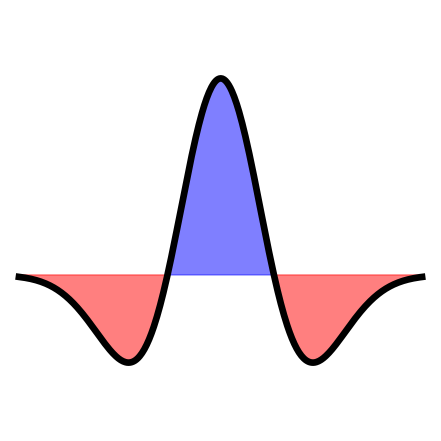
\includegraphics[width=7cm]{figures/icon}}
\version{2022.12}



\begin{document}

\maketitle

\newpage\null\thispagestyle{empty}\newpage

\begin{center}
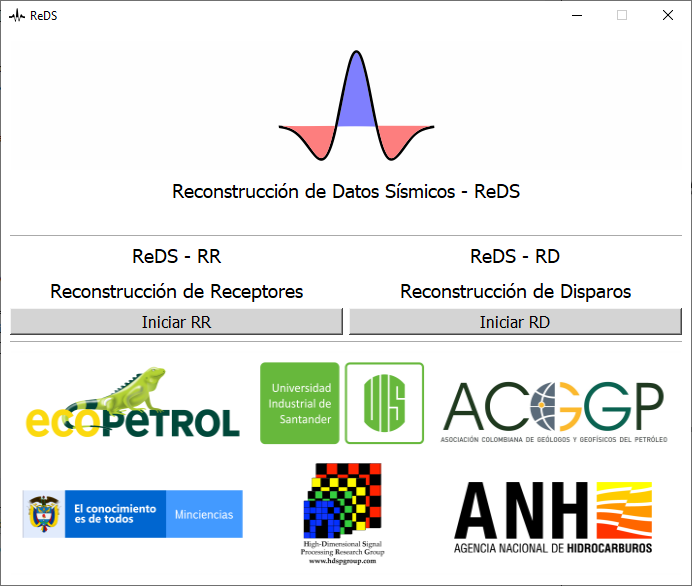
\includegraphics[width=.65\linewidth]{launch.png}
\end{center}
\begin{abstract}
%\includegraphics[width=1.0\linewidth]{PhysLogger.png}\\
%Esta aplicación pertenece al proyecto de investigación 9836, de la Universidad Industrial de Santander, Colombia. Esta aplicación permite la reconstrucción de trazas de muestras sísmicas mediante 4 diferentes algoritmos. Esta reconstrucción puede ser configurada por el usuario de tal manera que pueda realizar diferentes tipos de submuestreo y ajuste de parámetros mediante una interfaz gráfica de usuario.
La herramienta software Reconstrucción de Datos Sísmicos - ReDs hace parte del proyecto 9836 - ``Nuevas tecnologías computacionales para el diseño de sistemas de adquisición sísmica 3D terrestre con muestreo compresivo para la reducción de costos económicos e impactos ambientales en la exploración de hidrocarburos en cuencas terrestres colombianas''.

El proyecto 9836 está adscrito a la Convocatoria para la financiación de proyectos de investigación en geociencias para el sector de hidrocarburos, desarrollado por la alianza Universidad Industrial de Santander (UIS), ECOPETROL y la Asociación Colombiana de Geólogos y Geofísicos del Petróleo (ACGGP). 

Este proyecto es financiado por MINCIENCIAS y la Agencia Nacional de Hidrocarburos (ANH). Los derechos y licencias de uso sobre esta aplicación software están reservados a las entidades aportantes.
\end{abstract}

\newpage\null\thispagestyle{empty}\newpage

\clearpage
\tableofcontents

\clearpage

\newpage\null\thispagestyle{empty}\newpage

\section*{Presentación}\label{presentacion}
\addcontentsline{toc}{section}{\nameref{presentacion}}


La siguiente guía contiene un conjunto de ejemplos sobre el uso de la aplicación ReDs. Para la descripción detallada de cada uno de los elementos de la aplicación ReDs, y su interfaz gráfica, por favor sírvase revisar el \textit{Manual de Usuario} incluido con esta guía.

\section{Reconstrucción de Datos Sísmicos}

Este ejemplo ilustra como realizar la reconstrucción de datos sísmicos.

\begin{enumerate}
	
	\item Inicie la aplicación ReDs y en la pantalla de inicio escoja la opción \textit{Iniciar RR}.
	
	\begin{multicols}{2}		
		\item Ubique, en la parte superior de la aplicación, el botón del menú principal		
		\begin{Figure}
			\centering
			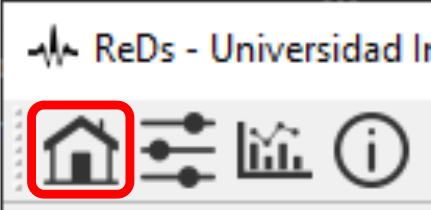
\includegraphics[width=0.4\linewidth]{main-tab.png}
			\captionof{figure}{Botón del menú principal.}
			\label{fig:main_button}
		\end{Figure}
	\end{multicols}

	\begin{multicols}{2}
		\begin{Figure}
			\centering
			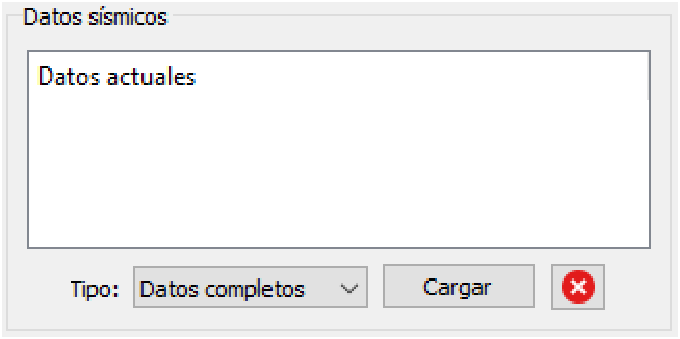
\includegraphics[width=.9\linewidth]{data-lecture-1.pdf}
			\captionof{figure}{Cargando un dato sísmico.}
			\label{fig:data_lecture_1}
		\end{Figure}
		\item En el extremo izquierdo, en el panel \textit{Datos Sísmicos}, haga click en el botón \textit{Cargar}
		\item En la ventana \textit{Abrir dato sísmico}, como se observa en la figura \ref{fig:data_lecture_2}, donde el usuario podrá seleccionar un dato sísmico. Para este ejemplo cargaremos \emph{data.npy}. La aplicación ReDs reconoce las extensiones \emph{.npy} y \emph{.mat} para cargar datos sísmicos.
	\end{multicols}

	\begin{Figure}
		\centering
		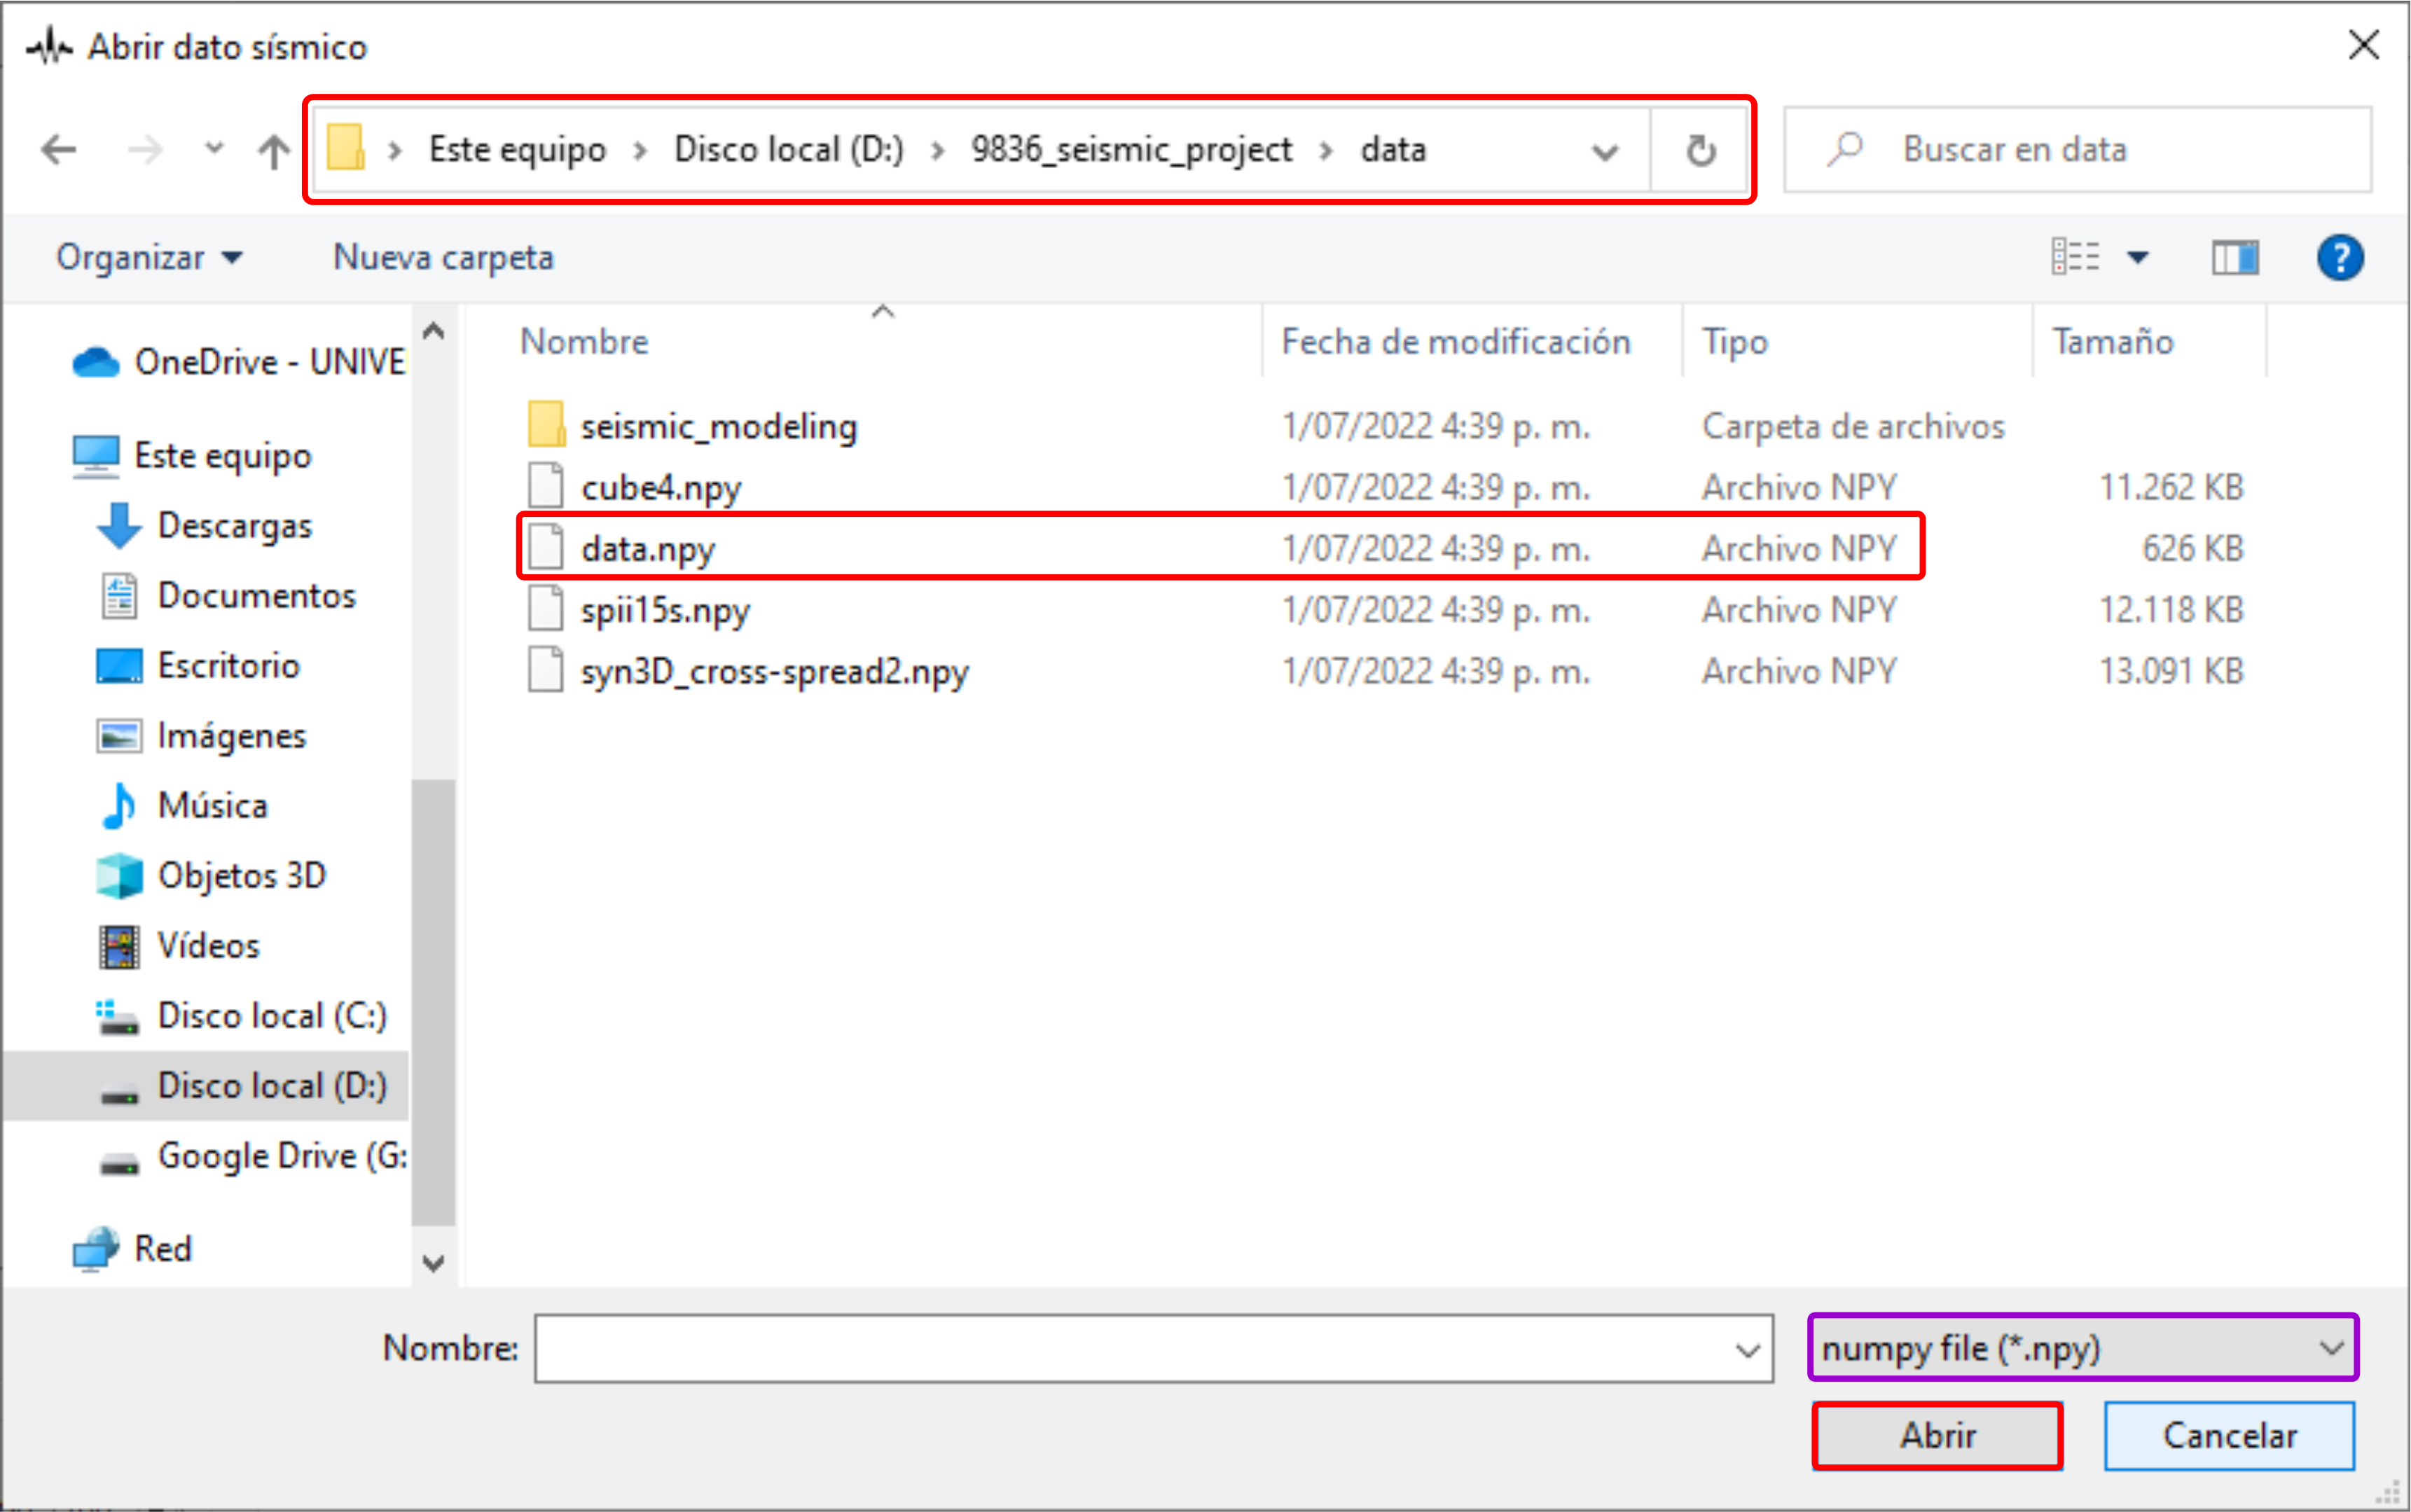
\includegraphics[width=1\linewidth]{data-lecture-2.png}
		\captionof{figure}{Ventana de selección de dato sísmico.}
		\label{fig:data_lecture_2}
	\end{Figure}

	\begin{multicols}{2}		
		\item En el panel \textit{Algoritmos}, extremo izquierdo, seleccione uno de los 4 algoritmos de reconstrucción. Para este ejemplo usaremos el algoritmo FISTA	y los valores de parámetros por defecto.
		\item En el mismo panel, establezca el valor de \textit{Máxima iteración} en 300.
		\item En el panel \textit{Submuestreo}, establezca el submuestro tipo \textit{Aleatorio} y una compresión del 50\%.
		\vfill\null
		\columnbreak
		\begin{Figure}
			\centering
			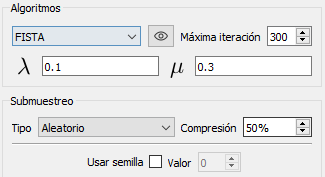
\includegraphics[width=0.95\linewidth]{example1.png}
			\captionof{figure}{Botón del menú principal.}
			\label{fig:example1}
		\end{Figure}
	\end{multicols}

	\begin{multicols}{2}
		\begin{Figure}
			\vspace{5mm}
			\centering
			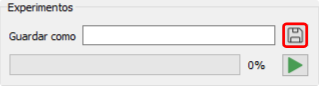
\includegraphics[width=0.9\linewidth]{experiment-1.png}
			\captionof{figure}{Panel de experimentos.}
			\label{fig:experiment_1}
		\end{Figure}		
		\item Seleccione un archivo para guardar los resultados de la reconstrucción con el botón \hspace{0.5mm} \faSave \hspace{0.5mm} ubicado en el panel \textit{Experimentos}. En la ventana \textit{Guardar reconstrucciones} introduzca el nombre \textit{nuevo\_experimento}, tal como se observa en la figura \ref{fig:experiment_2}.						
	\end{multicols}
	
	\begin{Figure}
		\centering
		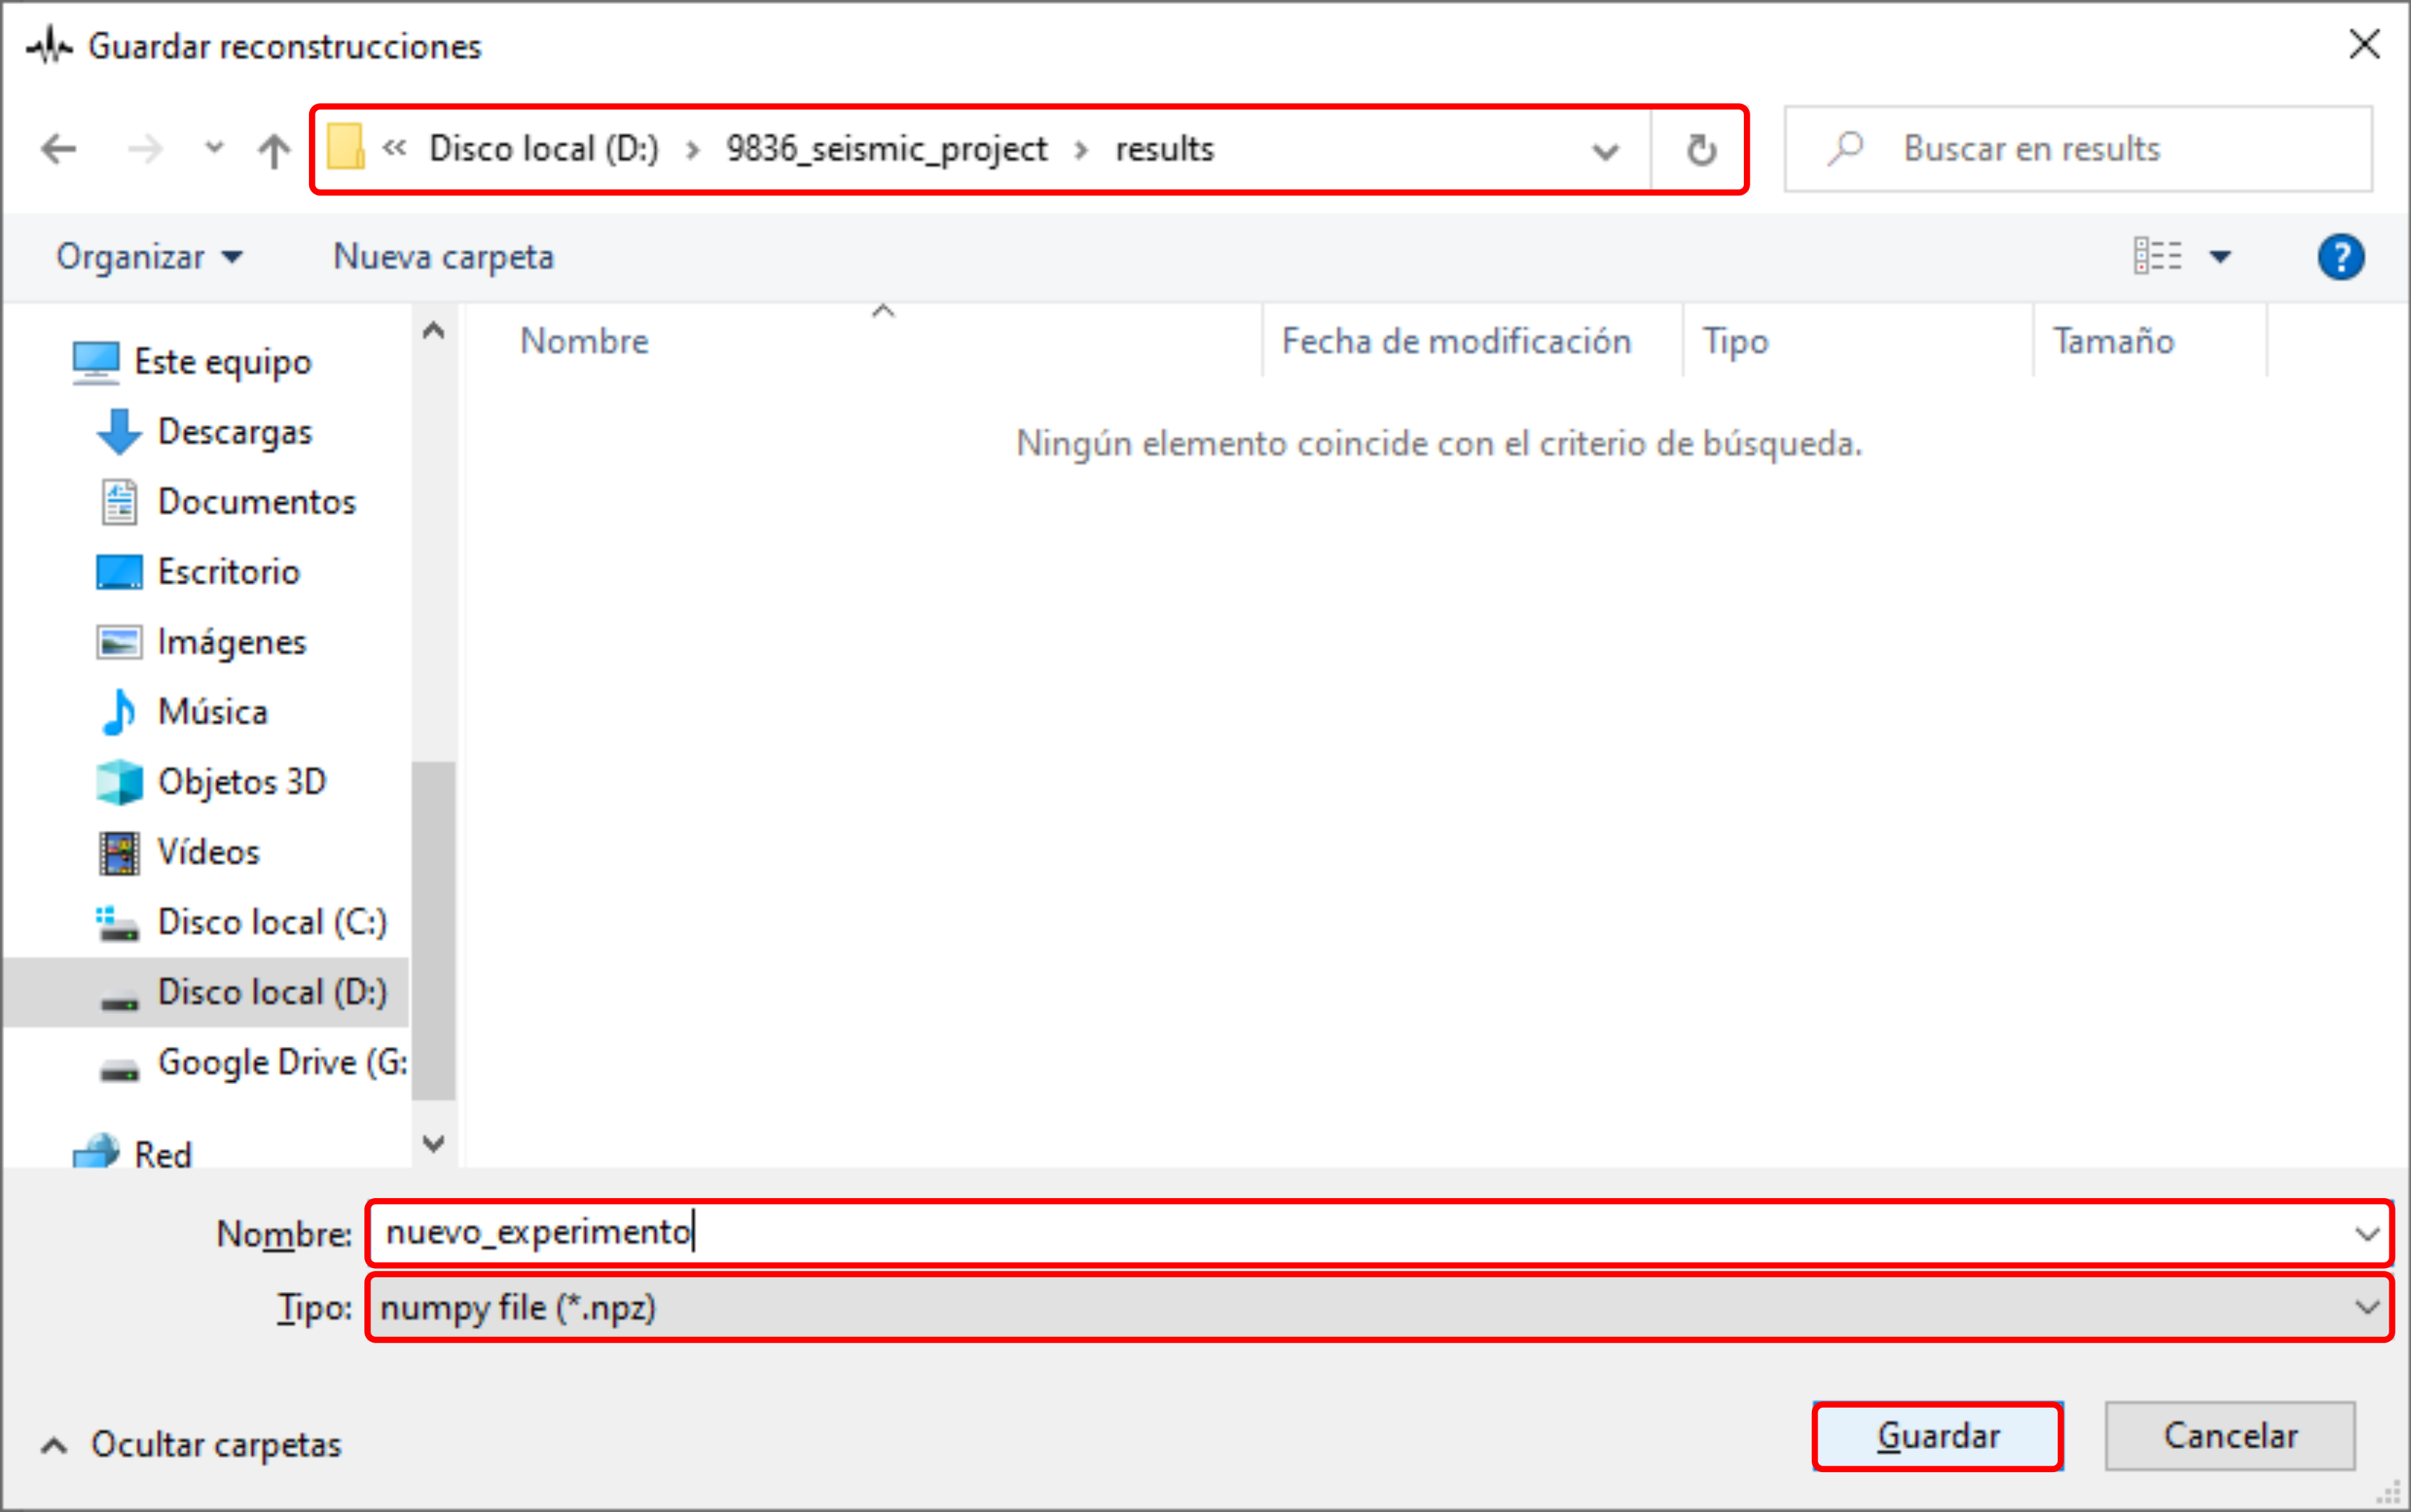
\includegraphics[width=1\linewidth]{experiment-2.png}
		\captionof{figure}{Ventana de guardado de resultados.}
		\label{fig:experiment_2}
	\end{Figure}

	\begin{multicols}{2}		
		\item Inicie la reconstrucción pulsando el botón \hspace{0.5mm} \faPlay \hspace{0.5mm}. En la barra de progreso, a la izquierda de dicho botón, se podrá el progreso del actual experimento, como se observa en la figura \ref{fig:experiment_4}.
		\begin{Figure}
			\centering
			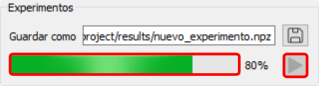
\includegraphics[width=0.7\linewidth]{experiment-4.png}
			\captionof{figure}{Ejecución de un experimento en tiempo real.}
			\label{fig:experiment_4}
		\end{Figure}		
	\end{multicols}

	\item Los resultados de la reconstrucción se presentan en el panel derecho de la apliación. En esta subventana se observa el rendimiento actual del experimento, como se muestra en la figura \ref{fig:main_result_2}, mediante una gráfica con dos ejes: el \textcolor{red}{eje izquierdo} representa el indice de similaridad estructural (SSIM); y el \textcolor{blue}{eje derecho} representa la proporción máxima de señal a ruido (PSNR) de las trazas reconstruidas con respecto a las verdaderas. En general, ambas métricas cuantifican la degradación de la calidad de la imagen.
	
	\begin{Figure}
		\centering
		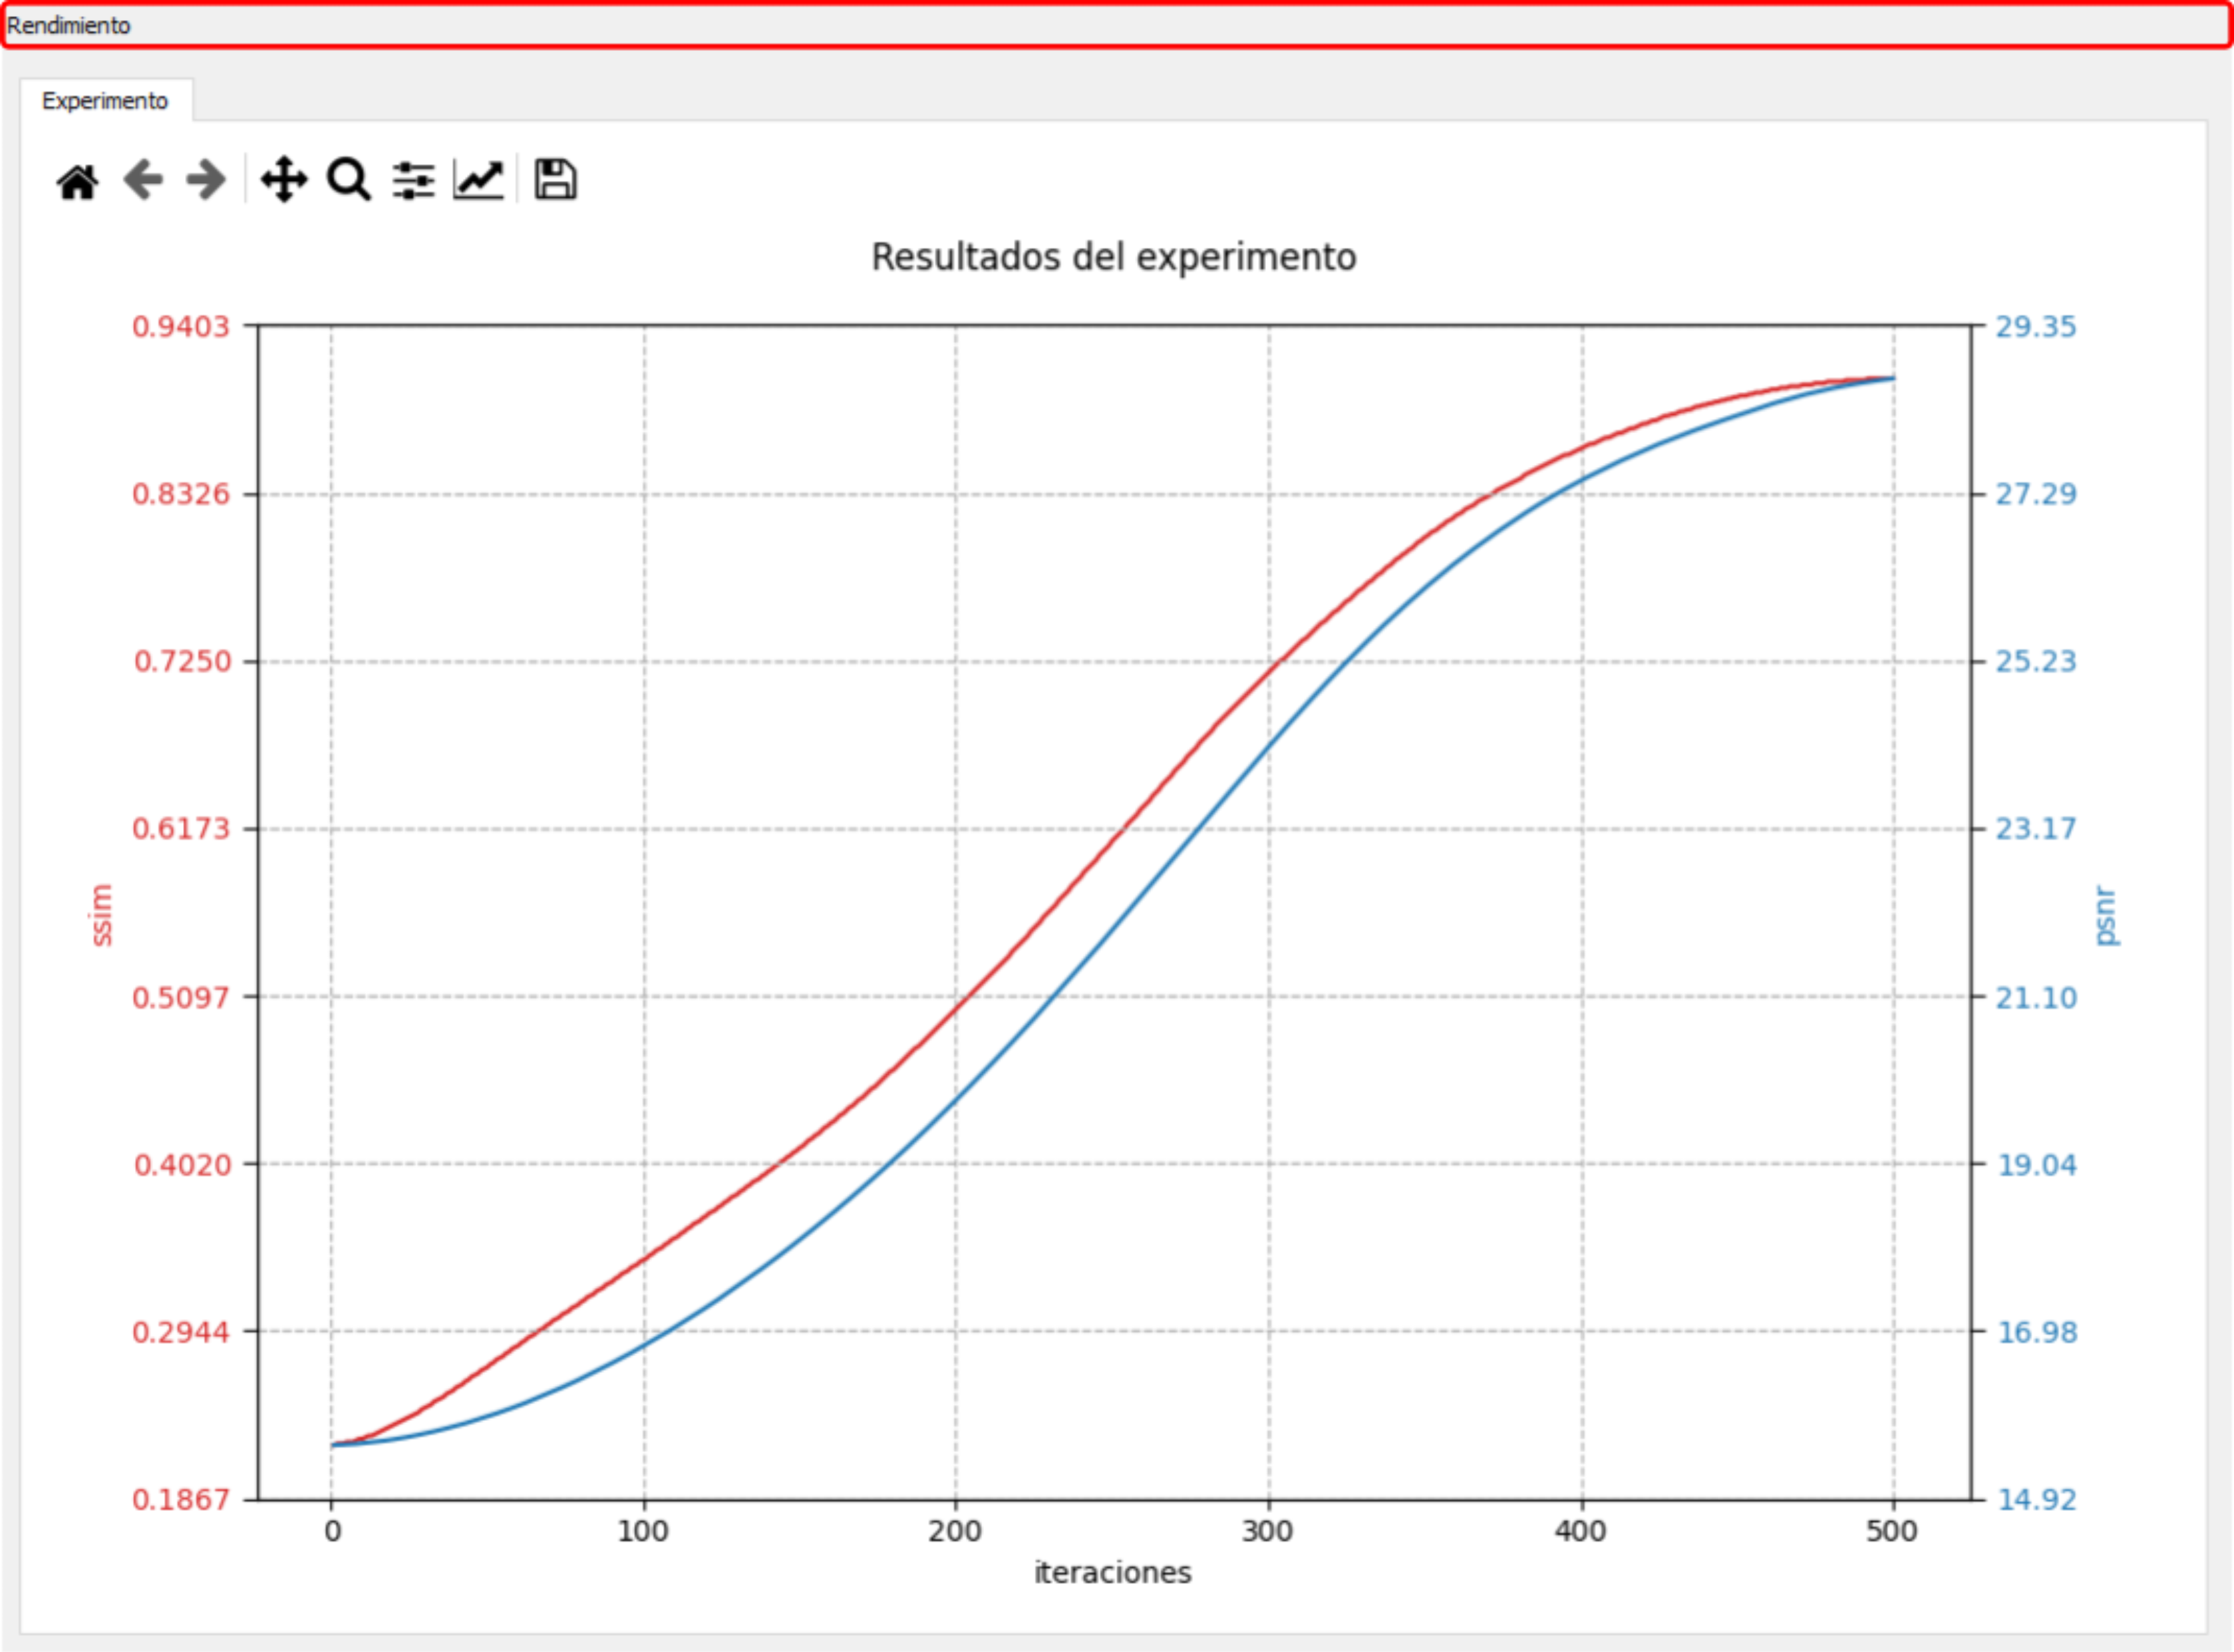
\includegraphics[width=0.8\linewidth]{main-result-2.png}
		\captionof{figure}{Rendimiento de un experimento realizado.}
		\label{fig:main_result_2}
	\end{Figure}

	\item Los resultados cuantitativos del experimento se observan en el subpanel de \emph{Reporte de Reconstrucción}, como se muestra en la figura \ref{fig:main_result_6}. Esta gráfica se divide en 4 secciones:
	
	\begin{itemize}[leftmargin=0.5in]
		\setlength\itemsep{0em}
		\item[I.]  \textit{Referencia}. Esta gráfica es el disparo sísmico completo, el cual se usa como referencia para comparar contra la reconstruida, tanto cuantitativa como cualitativamente.		
		\item[II.] \textit{Medidas}. Está gráfica es el disparo sísmico submuestreado, y es la que pasa a través de los algoritmos para reconstruir las líneas de receptores faltantes.		
		\item[III.] \textit{Reconstruido}. Está gráfica contiene el disparo sísmico reconstruida.		
		\item[IV.] \textit{Traza}. Esta gráfica contiene una de las trazas reconstruidas comparada contra la de referencia.		
	\end{itemize}

	\begin{Figure}
		\centering
		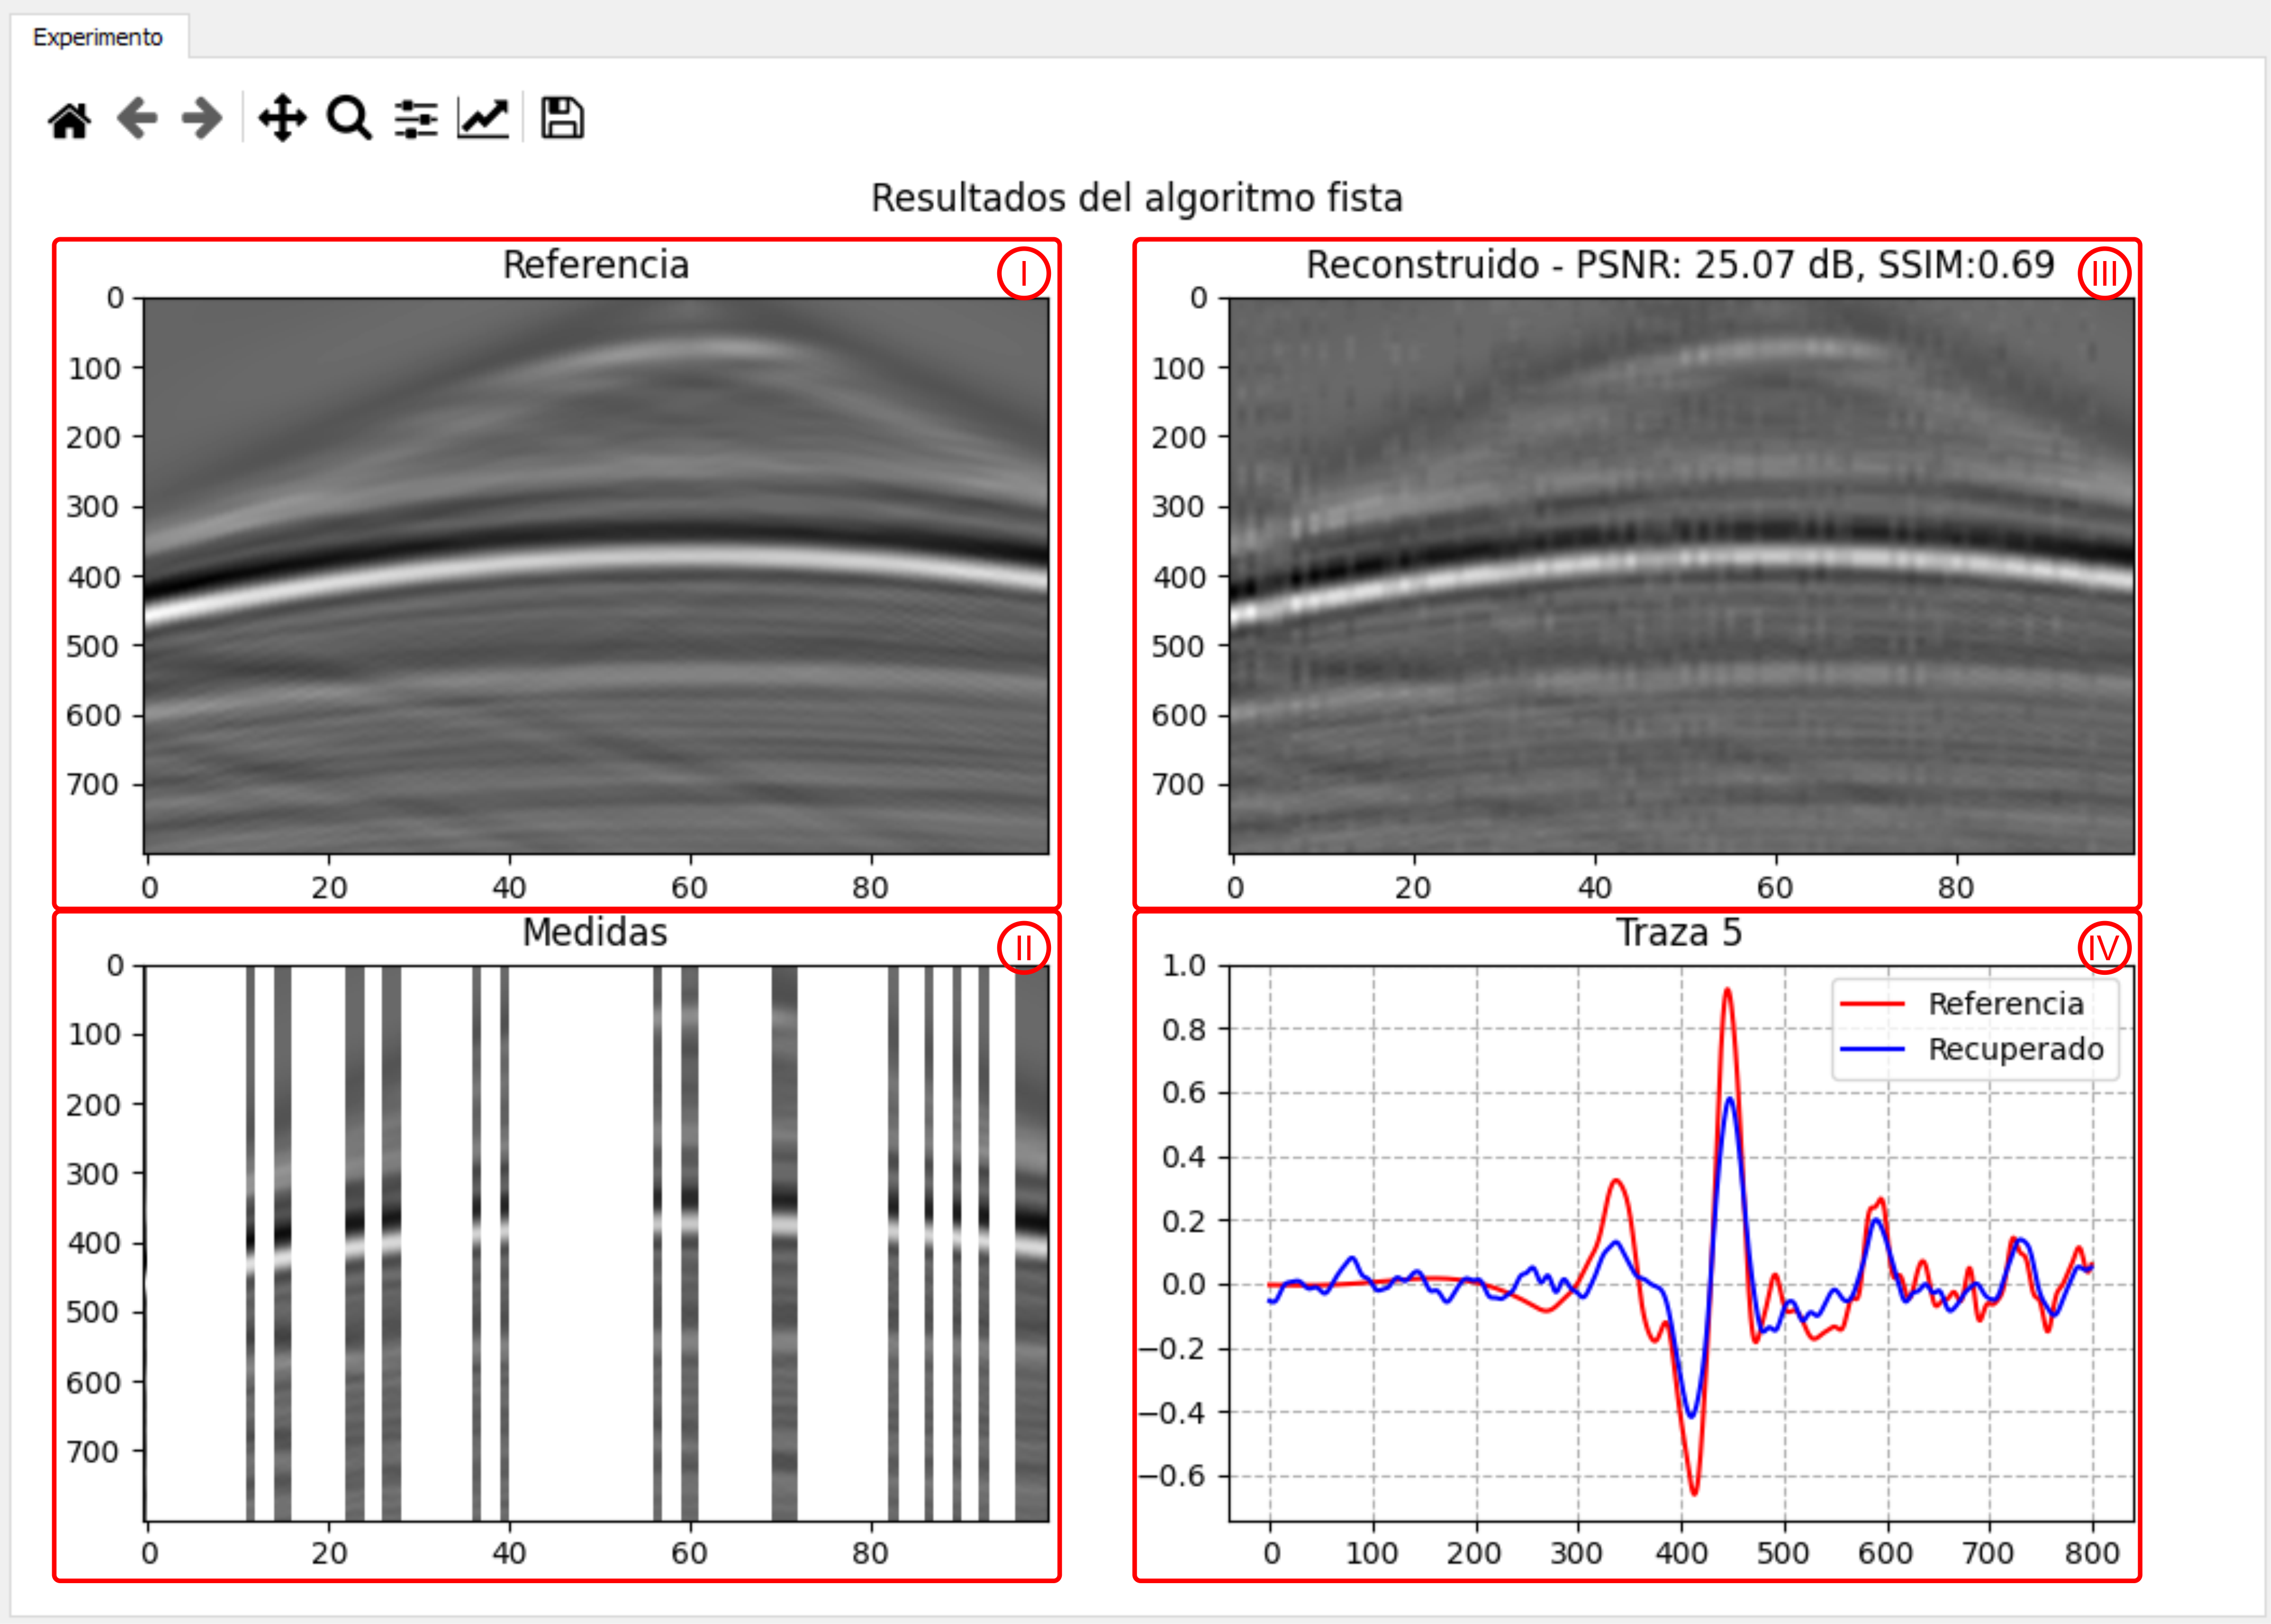
\includegraphics[width=1\linewidth]{main-result-6.png}
		\captionof{figure}{Reporte cuantitativo de un experimento realizado.}
		\label{fig:main_result_6}
	\end{Figure}

\end{enumerate}

\section{Ajuste de Parámetros}

Este ejemplo ilustra como realizar un ajuste de parámetros

\begin{enumerate}
	
	\item Inicie la aplicación ReDs y en la pantalla de inicio escoja la opción \textit{Iniciar RR}.
	
	\begin{multicols}{2}
		\item Ubique, en la parte superior de la aplicación, el botón del menú de ajuste de parámetros.
		\begin{Figure}			
			\centering
			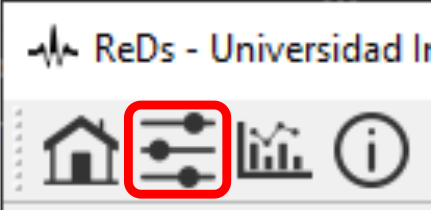
\includegraphics[width=0.4\linewidth]{tuning-tab.png}
			\captionof{figure}{Botón del menú de ajuste de parámetros.}
			\label{fig:tuning_button}
		\end{Figure}					
	\end{multicols}
	
	\begin{multicols}{2}
		\begin{Figure}
			\centering
			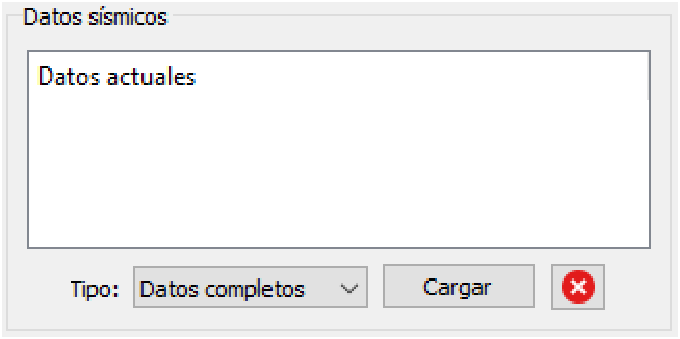
\includegraphics[width=.9\linewidth]{data-lecture-1.pdf}
			\captionof{figure}{Cargando un dato sísmico.}
			\label{fig:data_lecture_1a}
		\end{Figure}
		\item En el extremo izquierdo, en el panel \textit{Datos Sísmicos}, haga click en el botón \textit{Cargar}
		\item En la ventana \textit{Abrir dato sísmico}, como se observa en la figura \ref{fig:data_lecture_2}, donde el usuario podrá seleccionar un dato sísmico. Para este ejemplo cargaremos \emph{data.npy}. La aplicación ReDs reconoce las extensiones \emph{.npy} y \emph{.mat} para cargar datos sísmicos.
	\end{multicols}
	
	\begin{Figure}
		\centering
		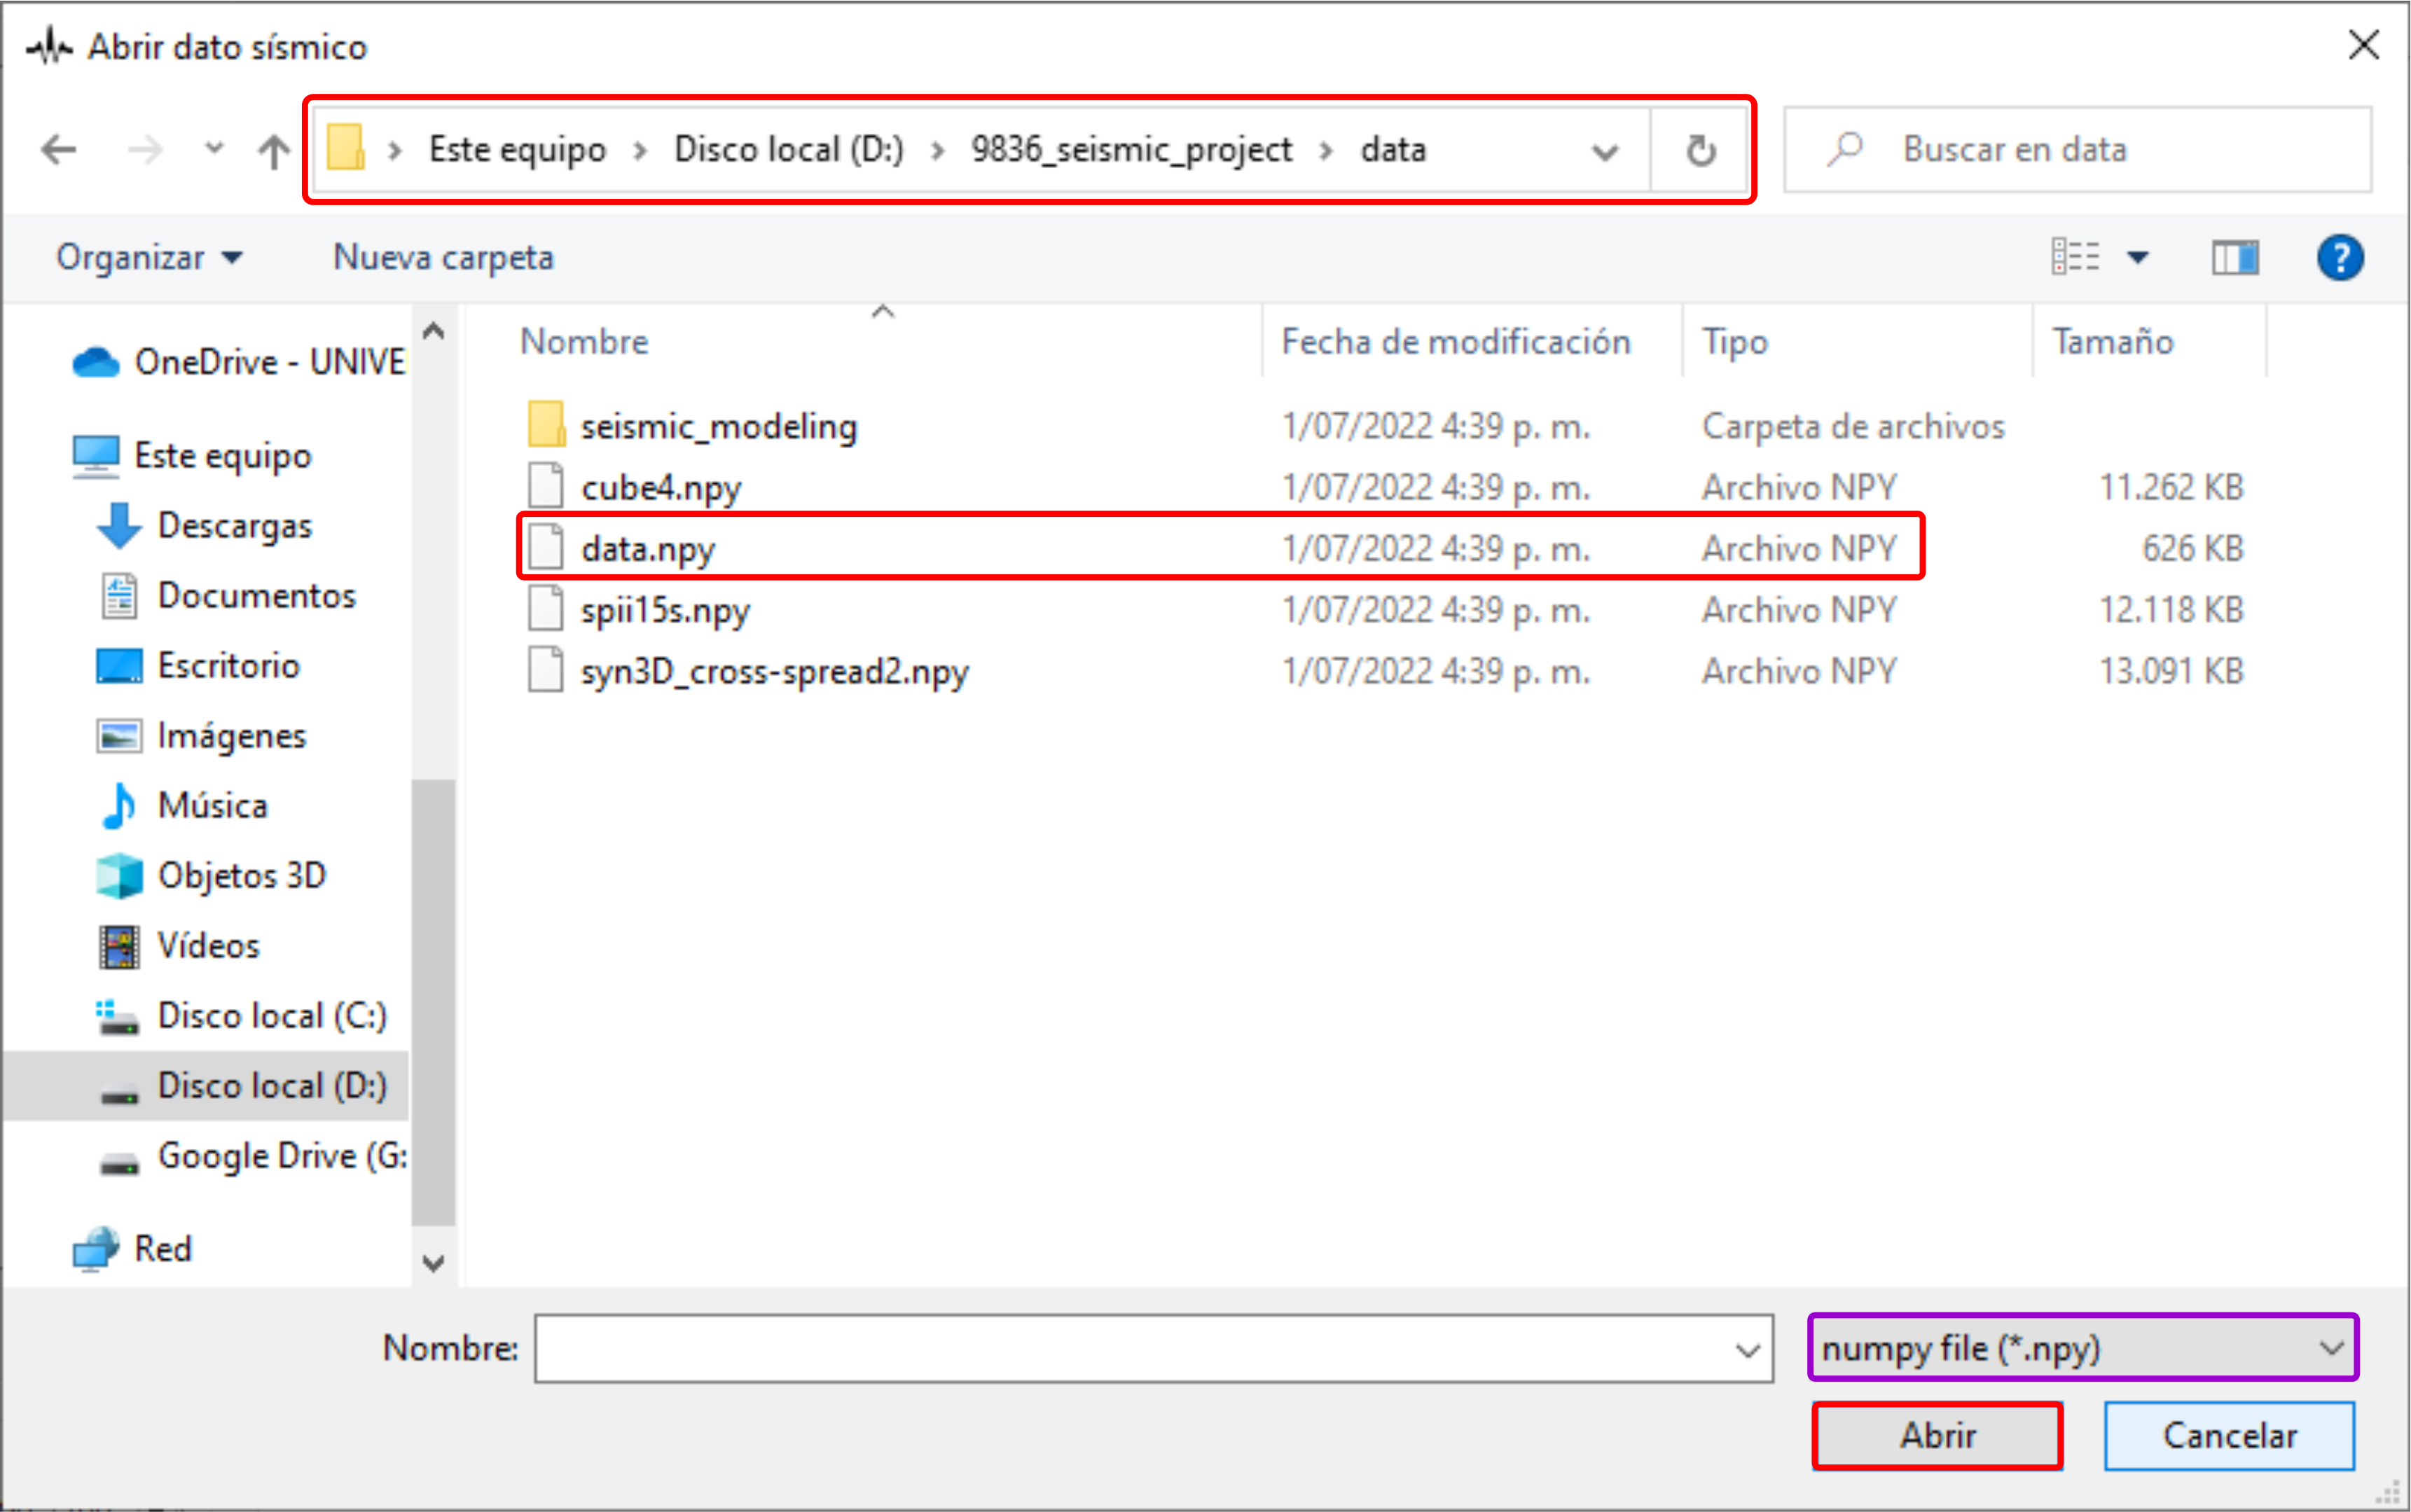
\includegraphics[width=1\linewidth]{data-lecture-2.png}
		\captionof{figure}{Ventana de selección de dato sísmico.}
		\label{fig:data_lecture_2a}
	\end{Figure}

	\begin{multicols}{2}
		\item En el panel izquierdo \textit{Algoritmo} escoja uno de los cuatro algoritmos de reconstrucción. Para este caso escogeremos FISTA.
		\item Establezca 300 iteraciones como valor máximo
		\vfill\null
		\columnbreak
		\begin{Figure}			
			\centering
			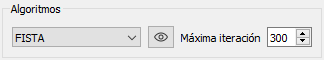
\includegraphics[width=0.85\linewidth]{example2.png}
			\captionof{figure}{Algoritmo a ajustar}
			\label{fig:algajuste}
		\end{Figure}					
	\end{multicols}

	\begin{multicols}{2}
		\begin{Figure}			
			\centering
			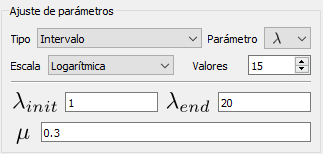
\includegraphics[width=0.85\linewidth]{example3.png}
			\captionof{figure}{Menú de ajuste de parámetros.}
			\label{fig:example3}
		\end{Figure}
		\vfill\null
		\columnbreak
		\item En el panel izquierdo \textit{Ajuste de parámetros} Cambie la opción \textit{Escala} a \textit{Logarítmica}, y la cantidad de \textit{Valores} a 15.
		\item Cambie el rango de valores del parámetro $ \lambda $, y el valor de $ \mu $, tal como se indica en la figura \ref{fig:example3}
	\end{multicols}

	\begin{multicols}{2}
		\item Seleccione un archivo para guardar los resultados de la reconstrucción con el botón \hspace{0.5mm} \faSave \hspace{0.5mm} ubicado en el panel \textit{Experimentos}. En la ventana \textit{Guardar reconstrucciones} introduzca el nombre \textit{nuevo\_experimento}, tal como se observa en la figura \ref{fig:experiment_2a}.
		\begin{Figure}
			\vspace{5mm}
			\centering
			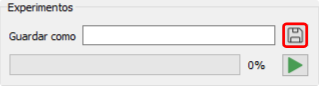
\includegraphics[width=0.9\linewidth]{experiment-1.png}
			\captionof{figure}{Panel de experimentos.}
			\label{fig:experiment_1a}
		\end{Figure}								
	\end{multicols}
	
	\begin{Figure}
		\centering
		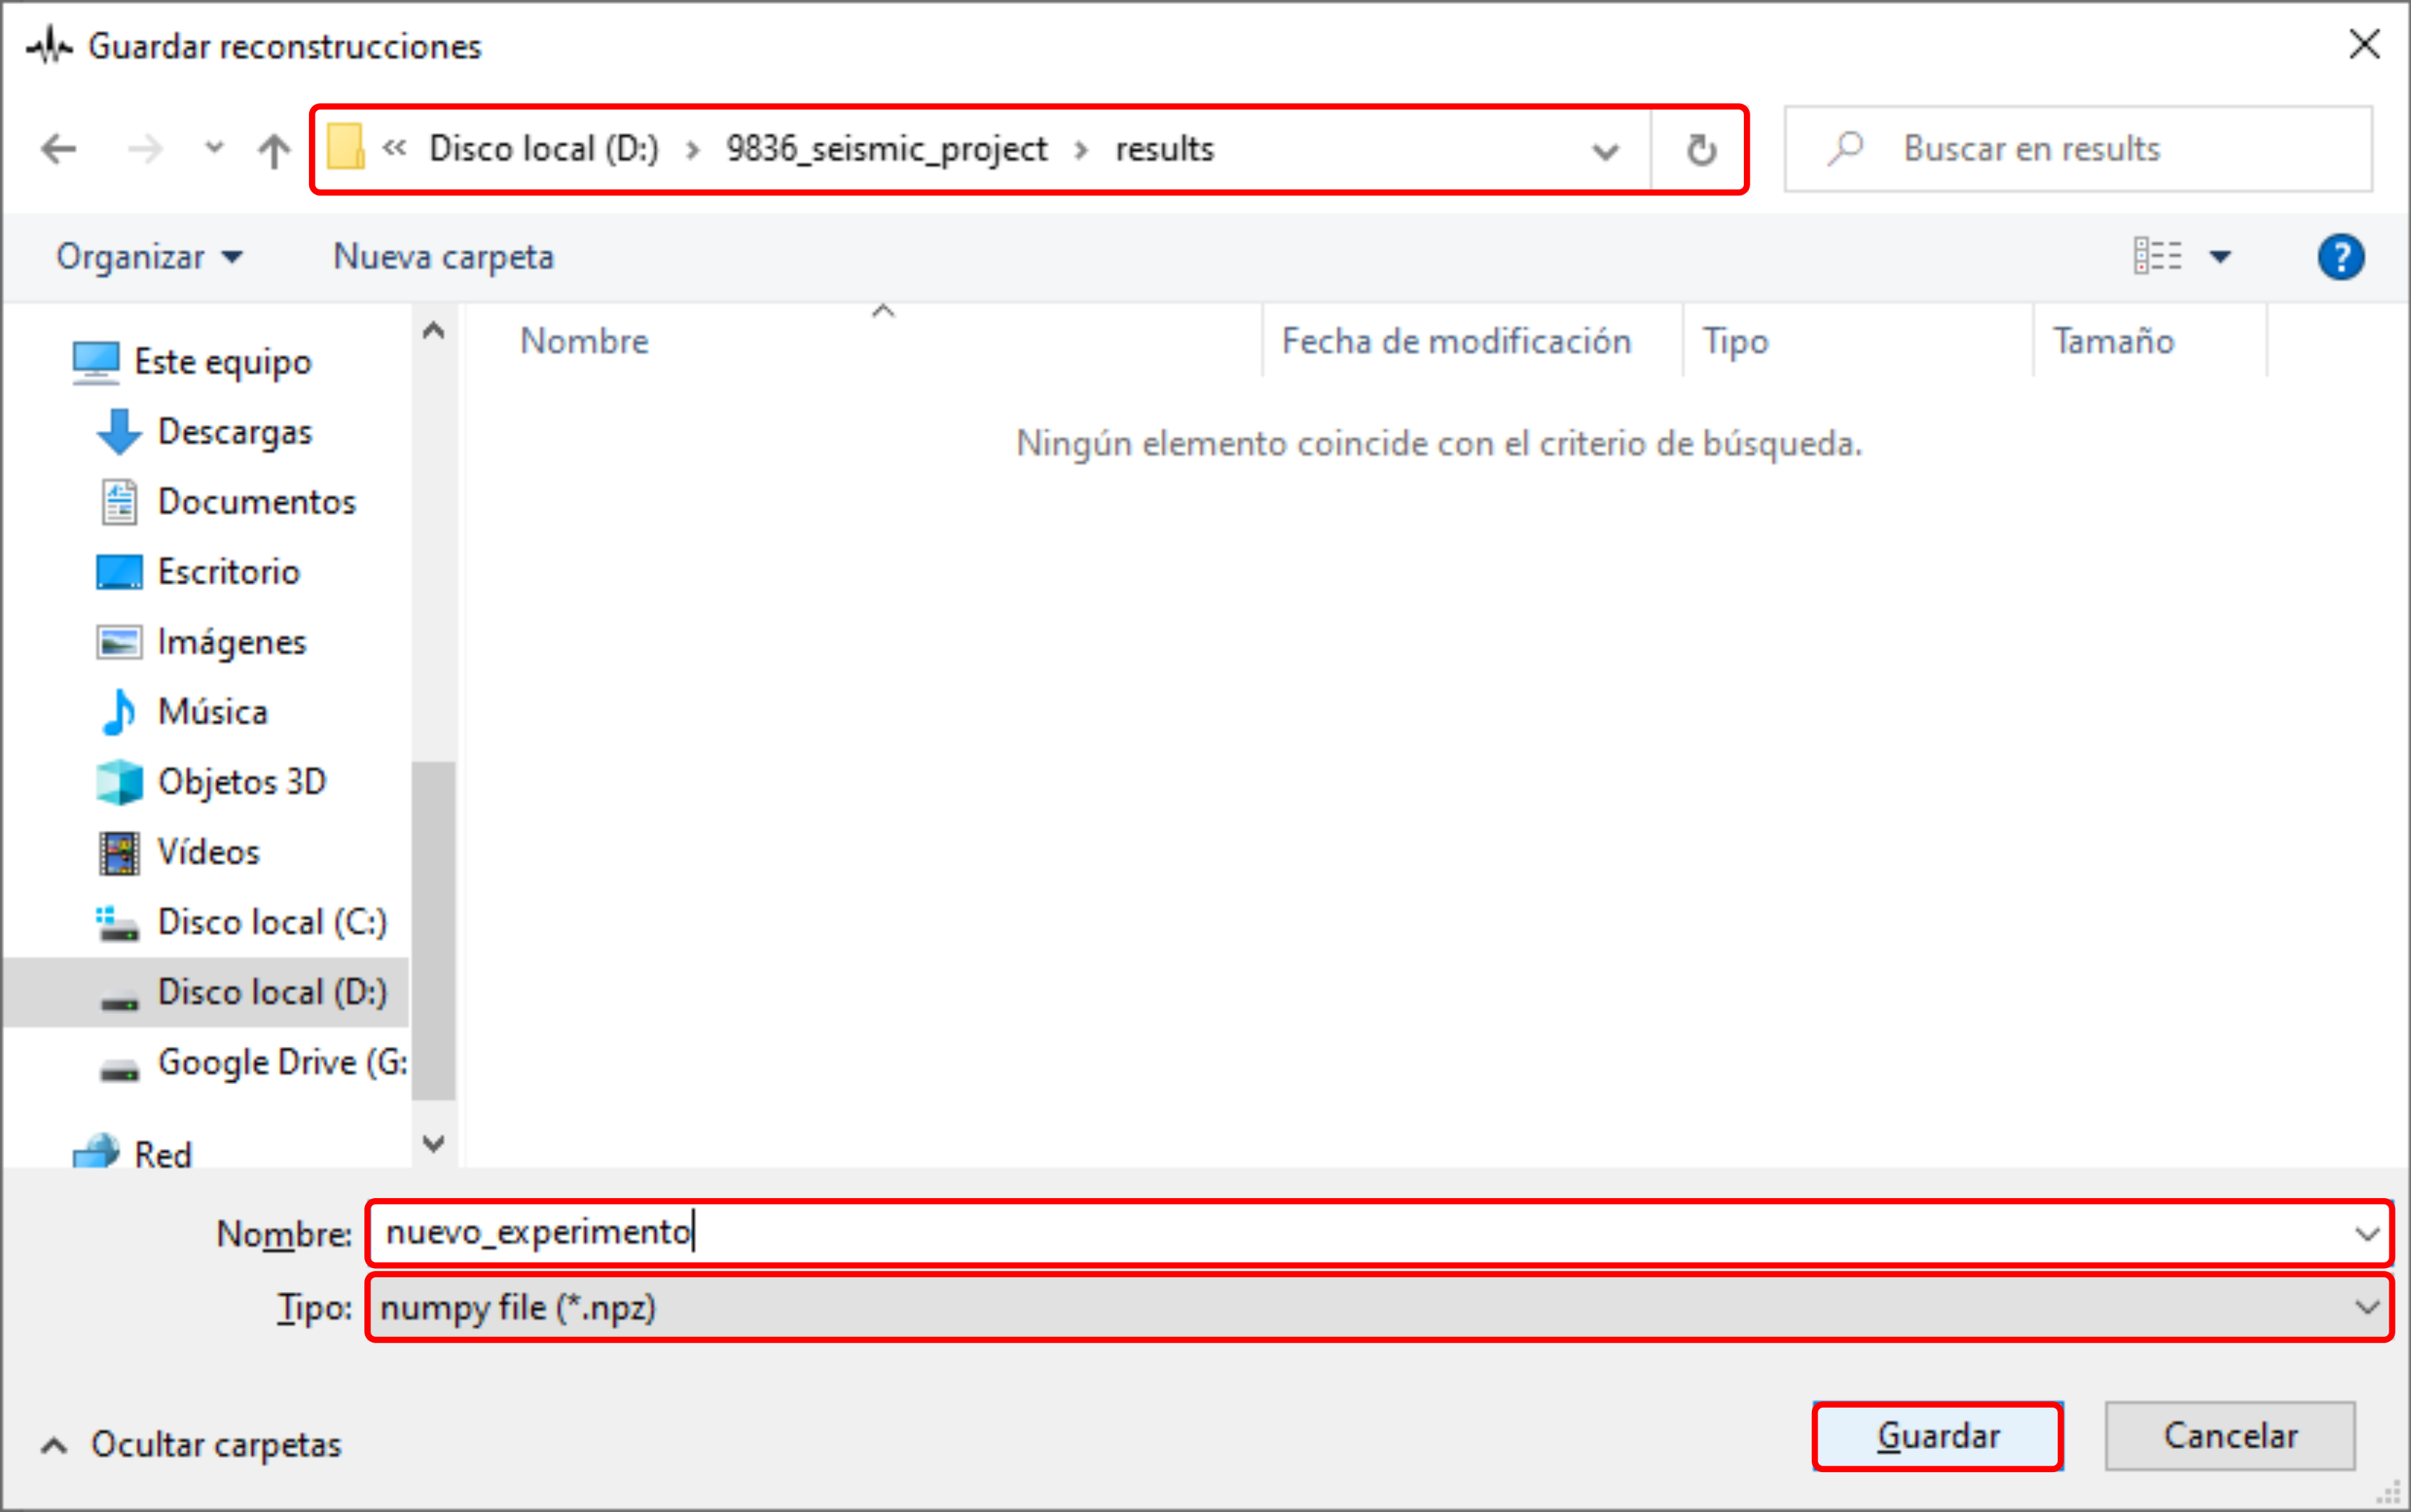
\includegraphics[width=1\linewidth]{experiment-2.png}
		\captionof{figure}{Ventana de guardado de resultados.}
		\label{fig:experiment_2a}
	\end{Figure}
	
	\begin{multicols}{2}
		\begin{Figure}
			\centering
			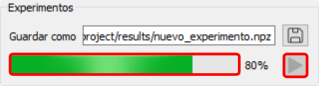
\includegraphics[width=0.7\linewidth]{experiment-4.png}
			\captionof{figure}{Ejecución de un experimento en tiempo real.}
			\label{fig:experiment_4a}
		\end{Figure}		
		\item Inicie la reconstrucción pulsando el botón \hspace{0.5mm} \faPlay \hspace{0.5mm}. En la barra de progreso, a la izquierda de dicho botón, se podrá el progreso del actual experimento, como se observa en la figura \ref{fig:experiment_4a}.				
	\end{multicols}

	\item Los resultados obtenidos para este ajuste de parámetros se observan en la figura \ref{fig:tuning_2}. Por inspección, se observa que el valor óptimo $\mu^* \approx 0.39$.
	
	\begin{Figure}
	\centering
	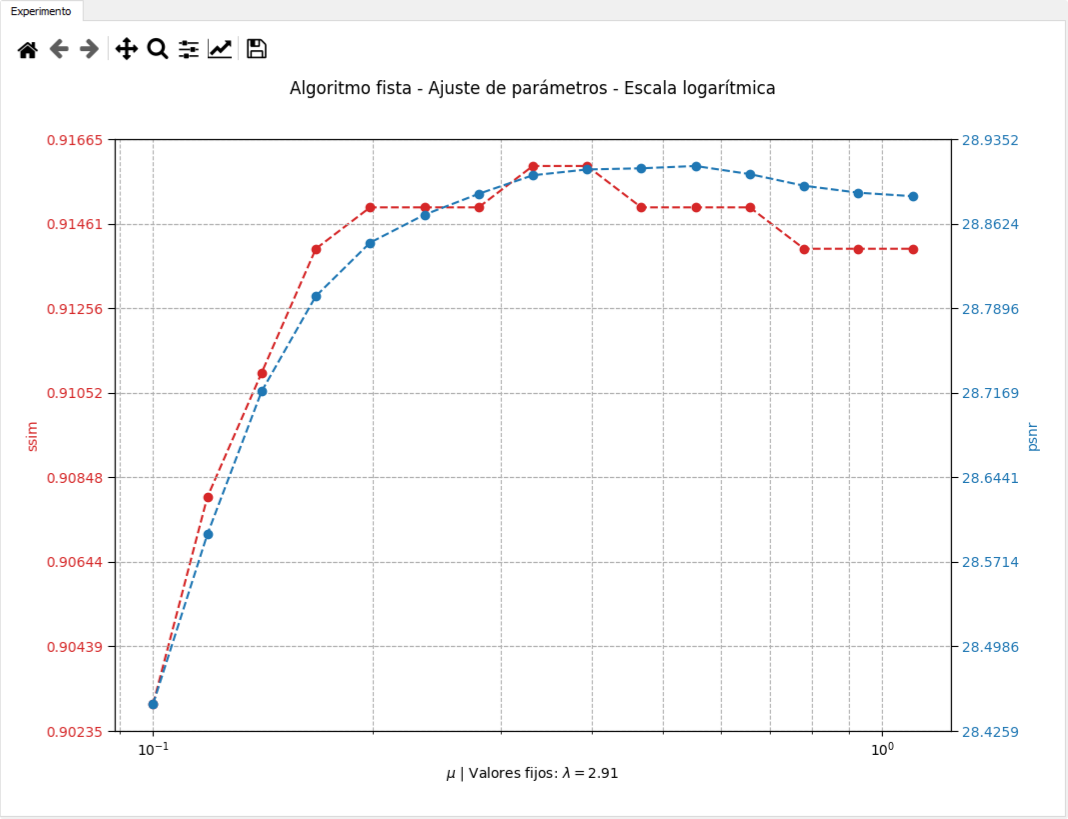
\includegraphics[width=1\linewidth]{tuning-2.png}
	\captionof{figure}{Ajuste del parámetro $\mu$ para el algoritmo FISTA.}
	\label{fig:tuning_2}
	\end{Figure}

\end{enumerate}

\section{Comparación de Algoritmos}

Este ejemplo ilustra como realizar una comparación de algoritmos

\begin{enumerate}
	
	\item Inicie la aplicación ReDs y en la pantalla de inicio escoja la opción \textit{Iniciar RR}.
	
	\begin{multicols}{2}
		\item Ubique, en la parte superior de la aplicación, el botón del menú de comparación de algoritmos.
		\begin{Figure}
			\centering
			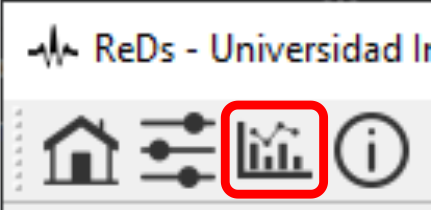
\includegraphics[width=0.4\linewidth]{comp-tab.png}
			\captionof{figure}{Modo de comparación de algoritmos.}
			\label{fig:comp}
		\end{Figure}					
	\end{multicols}

	\begin{multicols}{2}
		\begin{Figure}
			\centering
			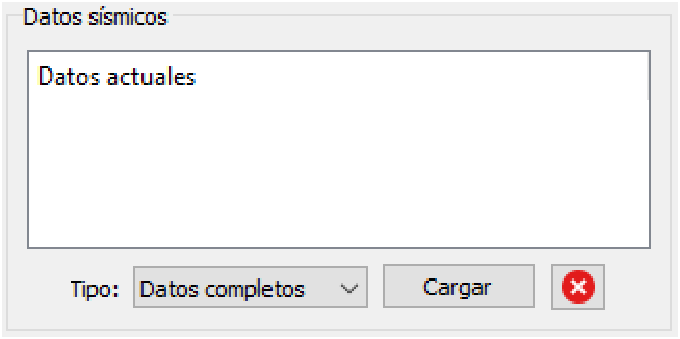
\includegraphics[width=.9\linewidth]{data-lecture-1.pdf}
			\captionof{figure}{Cargando un dato sísmico.}
			\label{fig:data_lecture_1b}
		\end{Figure}
		\item En el extremo izquierdo, en el panel \textit{Datos Sísmicos}, haga click en el botón \textit{Cargar}
		\item En la ventana \textit{Abrir dato sísmico}, como se observa en la figura \ref{fig:data_lecture_2b}, donde el usuario podrá seleccionar un dato sísmico. Para este ejemplo cargaremos \emph{data.npy}. La aplicación ReDs reconoce las extensiones \emph{.npy} y \emph{.mat} para cargar datos sísmicos.
	\end{multicols}
	
	\begin{Figure}
		\centering
		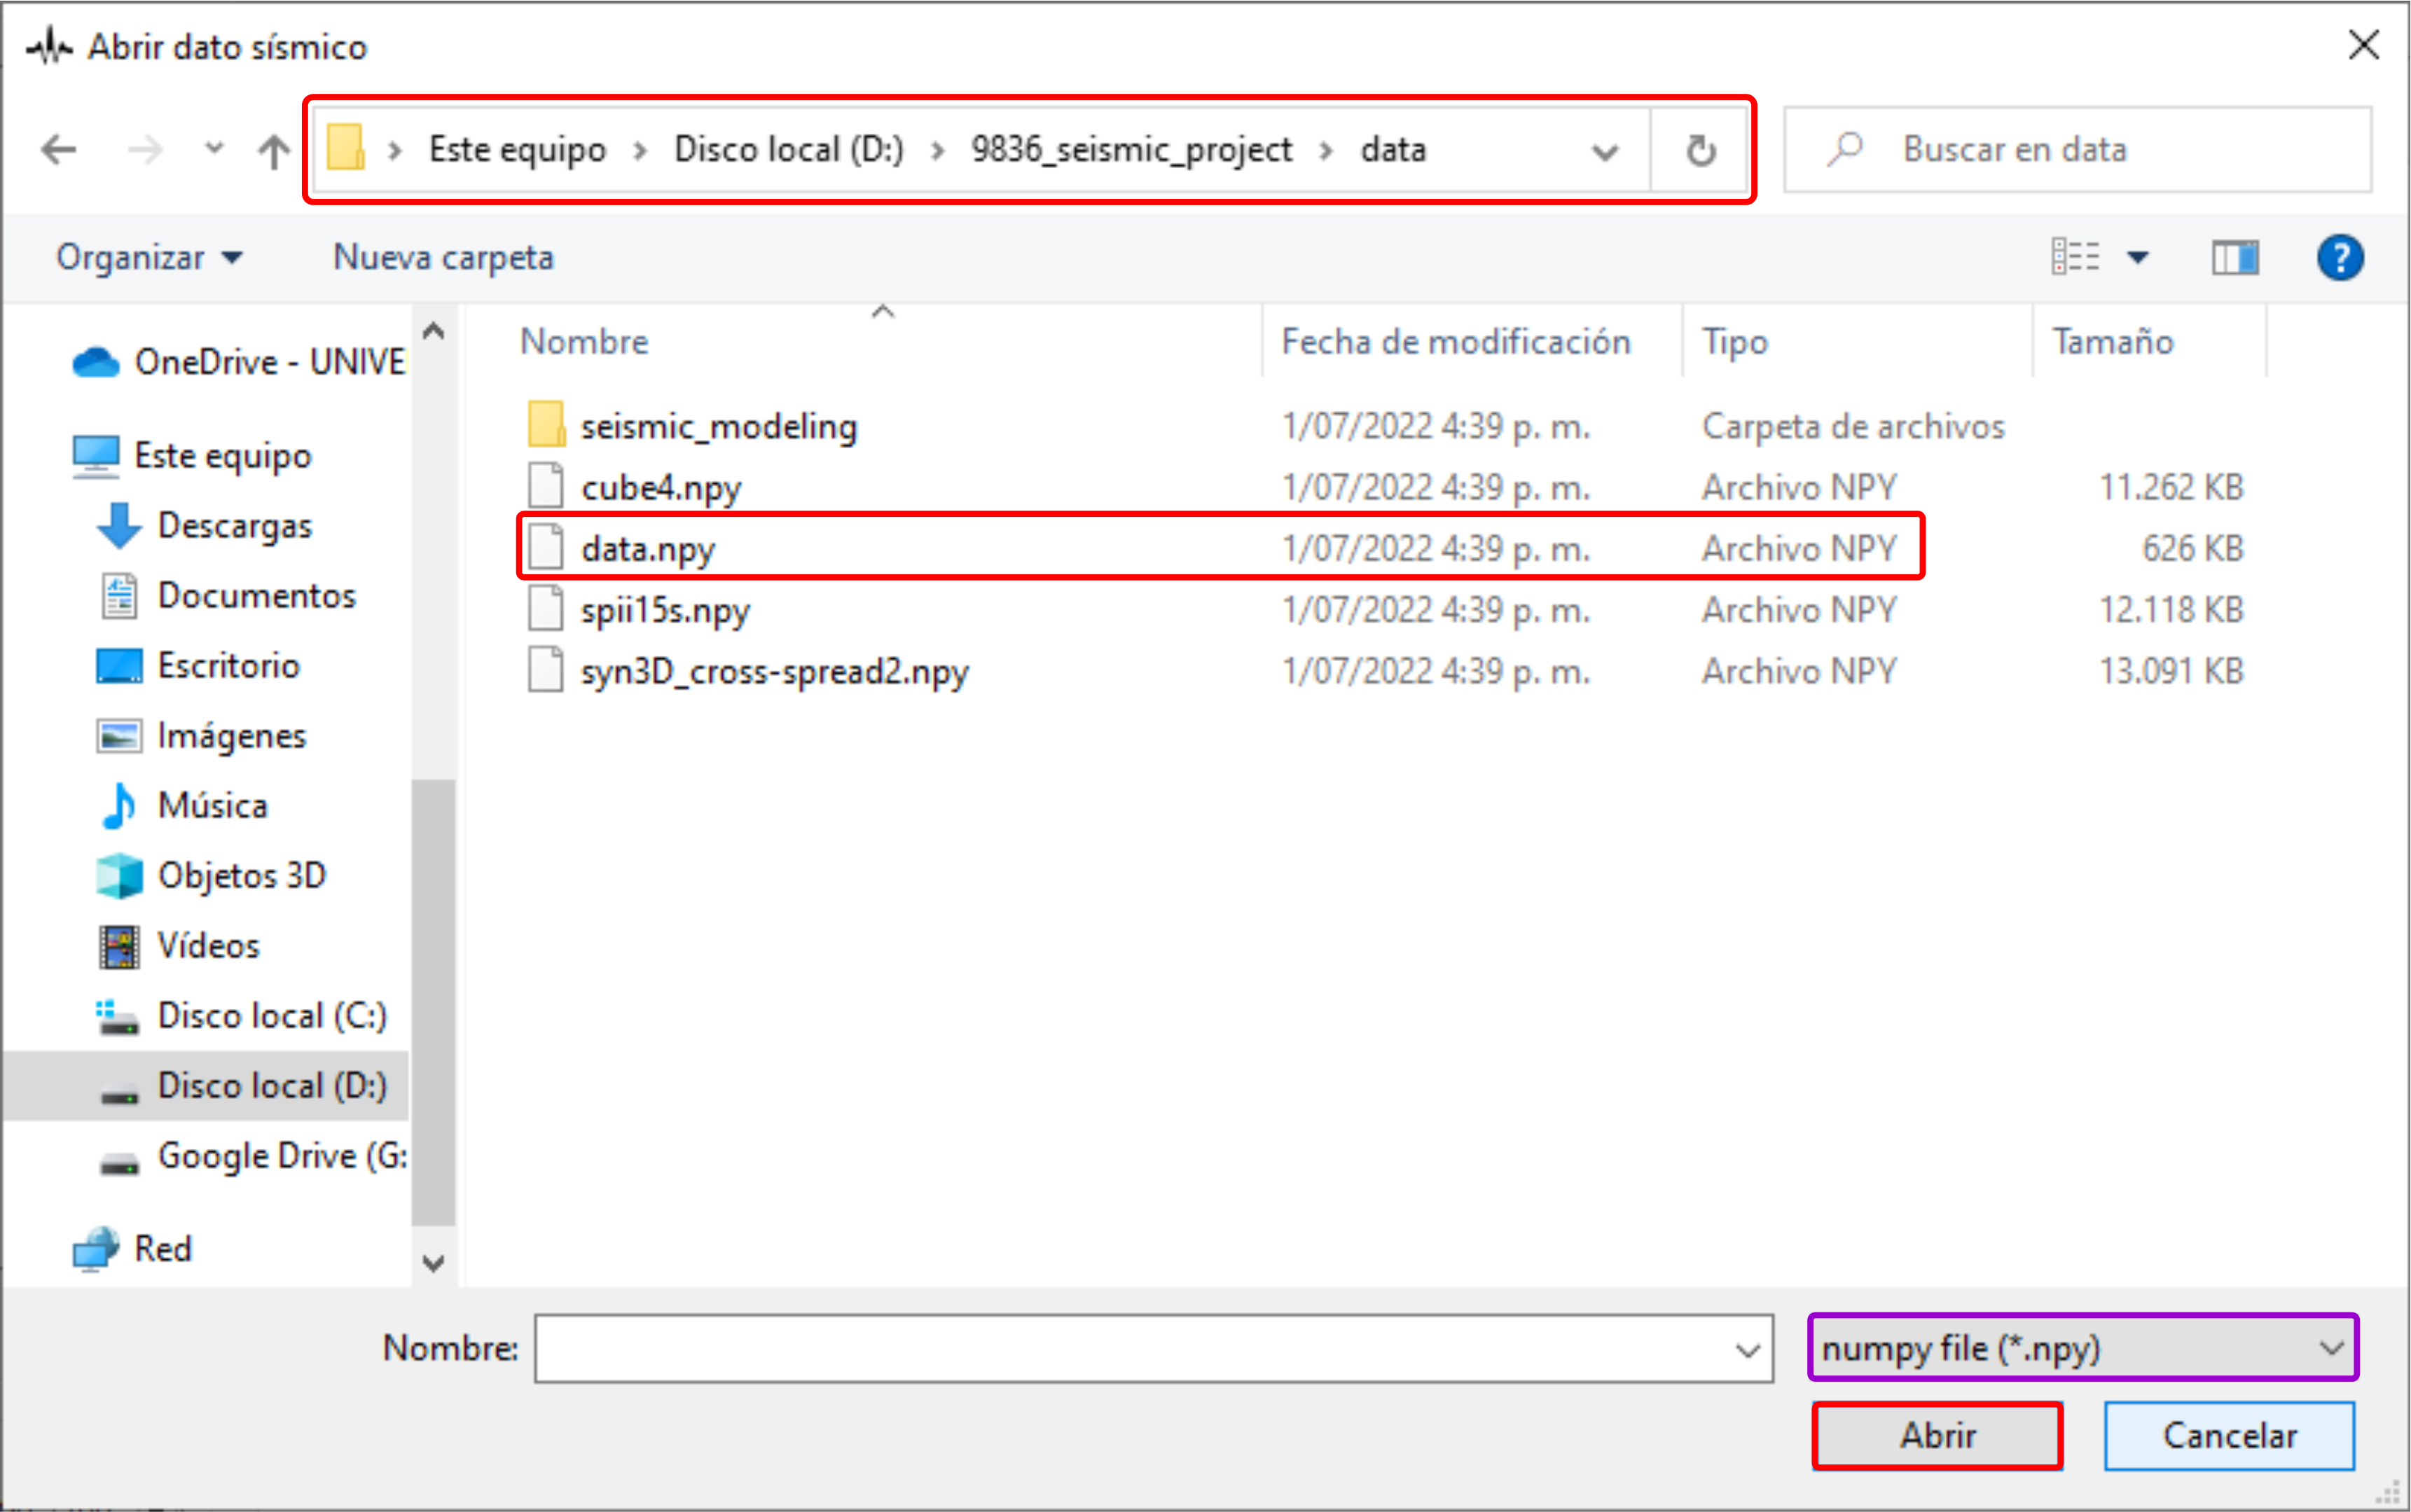
\includegraphics[width=1\linewidth]{data-lecture-2.png}
		\captionof{figure}{Ventana de selección de dato sísmico.}
		\label{fig:data_lecture_2b}
	\end{Figure}

	\begin{multicols}{2}
		\item En el panel derecho \textit{Comparaciones} mantenga la configuración por defecto. Puede cambiarlos valores para cada uno de los parámetros de los cuatro algoritmos de reconstrucción. En total son 9 parámetros a establecer: 2 para FISTA, 1 para GAP, 3 para TwIST y 3 para ADMM.
		\begin{Figure}
			\centering
			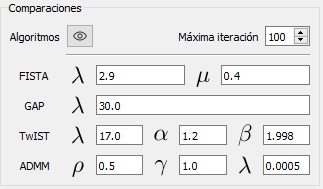
\includegraphics[width=0.85\linewidth]{example4.png}
			\captionof{figure}{Configuración de algoritmos.}
			\label{example4}
		\end{Figure}					
	\end{multicols}

	\begin{multicols}{2}
		\begin{Figure}
			\vspace{5mm}
			\centering
			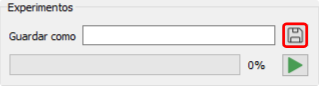
\includegraphics[width=0.9\linewidth]{experiment-1.png}
			\captionof{figure}{Panel de experimentos.}
			\label{fig:experiment_1b}
		\end{Figure}
		\item Seleccione un archivo para guardar los resultados de la reconstrucción con el botón \hspace{0.5mm} \faSave \hspace{0.5mm} ubicado en el panel \textit{Experimentos}. En la ventana \textit{Guardar reconstrucciones} introduzca el nombre \textit{nuevo\_experimento}, tal como se observa en la figura \ref{fig:experiment_2b}.								
	\end{multicols}
	
	\begin{Figure}
		\centering
		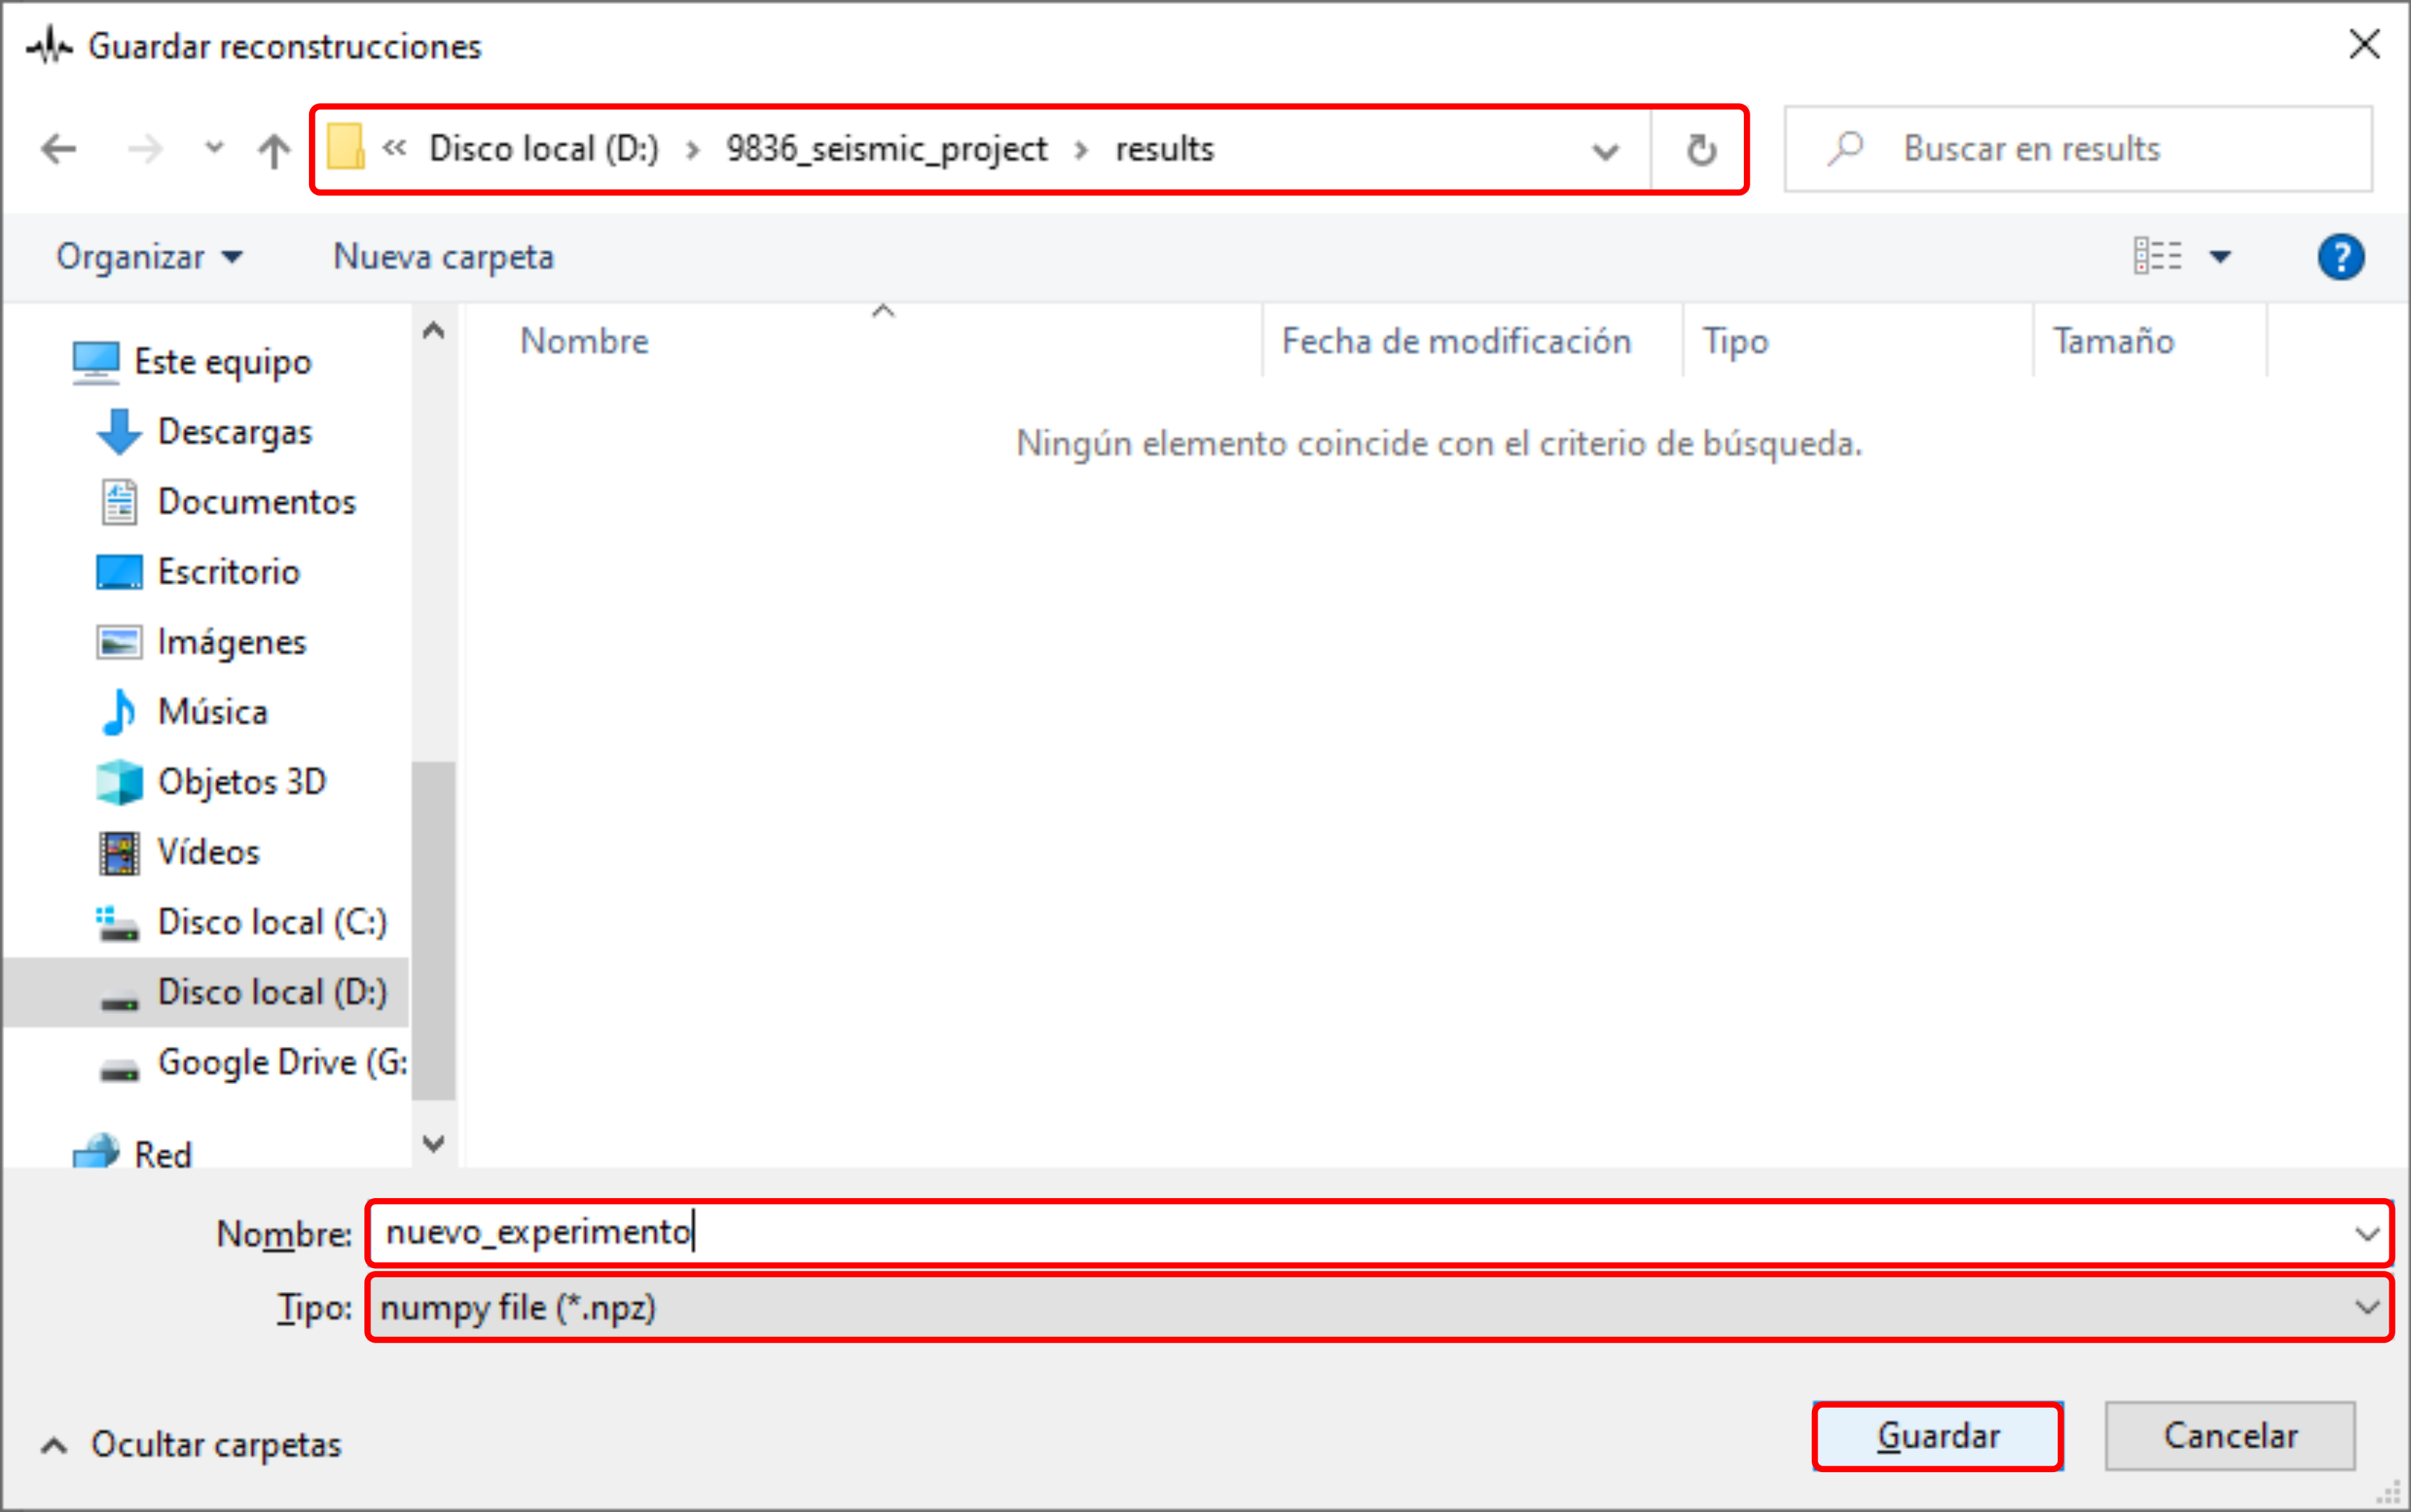
\includegraphics[width=1\linewidth]{experiment-2.png}
		\captionof{figure}{Ventana de guardado de resultados.}
		\label{fig:experiment_2b}
	\end{Figure}
	
	\begin{multicols}{2}
		\item Inicie la reconstrucción pulsando el botón \hspace{0.5mm} \faPlay \hspace{0.5mm}. En la barra de progreso, a la izquierda de dicho botón, se podrá el progreso del actual experimento, como se observa en la figura \ref{fig:experiment_4b}.		
		\begin{Figure}
			\centering
			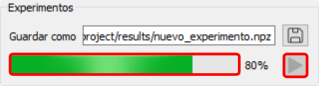
\includegraphics[width=0.7\linewidth]{experiment-4.png}
			\captionof{figure}{Ejecución de un experimento en tiempo real.}
			\label{fig:experiment_4b}
		\end{Figure}
	\end{multicols}

	\item La solución de la comparación de algoritmos se presenta en las pestañas Rendimiento y Reporte de reconstrucción, tal como se muestra en las figuras \ref{fig:result-comp1} y \ref{fig:result-comp2} respectivamente.
	
	\begin{Figure}
		\centering
		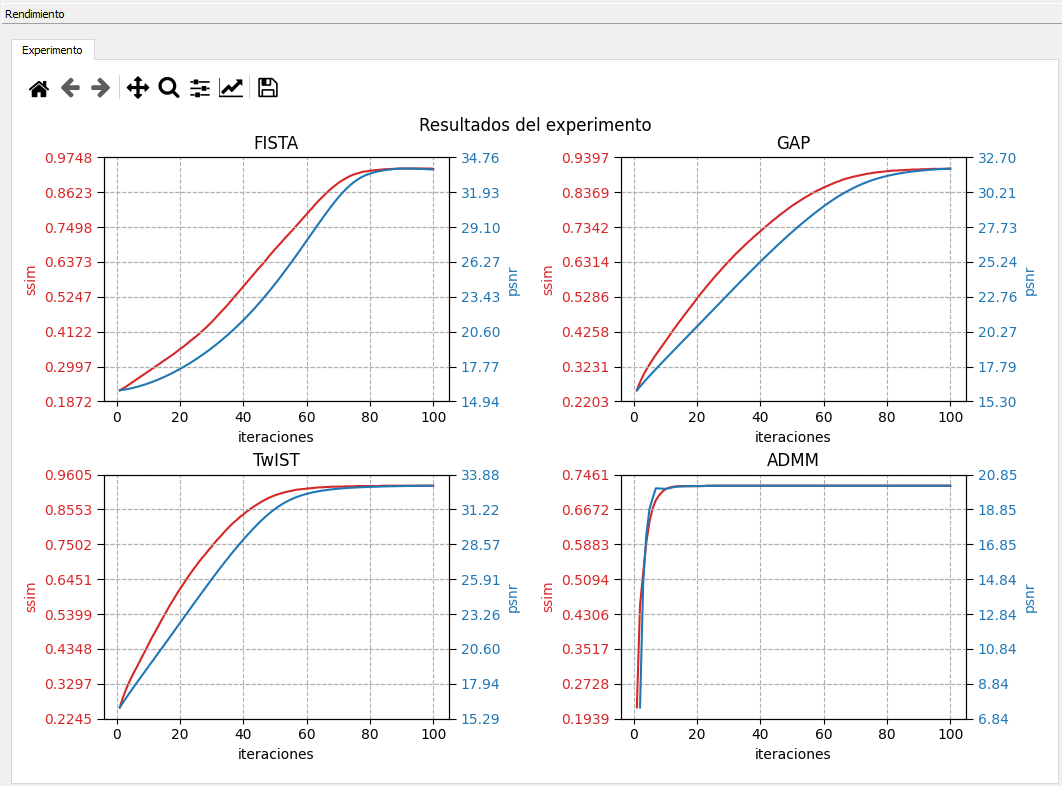
\includegraphics[width=0.9\linewidth]{result-comp1.png}
		\captionof{figure}{Rendimiento de la comparación de algoritmos}
		\label{fig:result-comp1}
	\end{Figure}
	
	\begin{Figure}
		\centering
		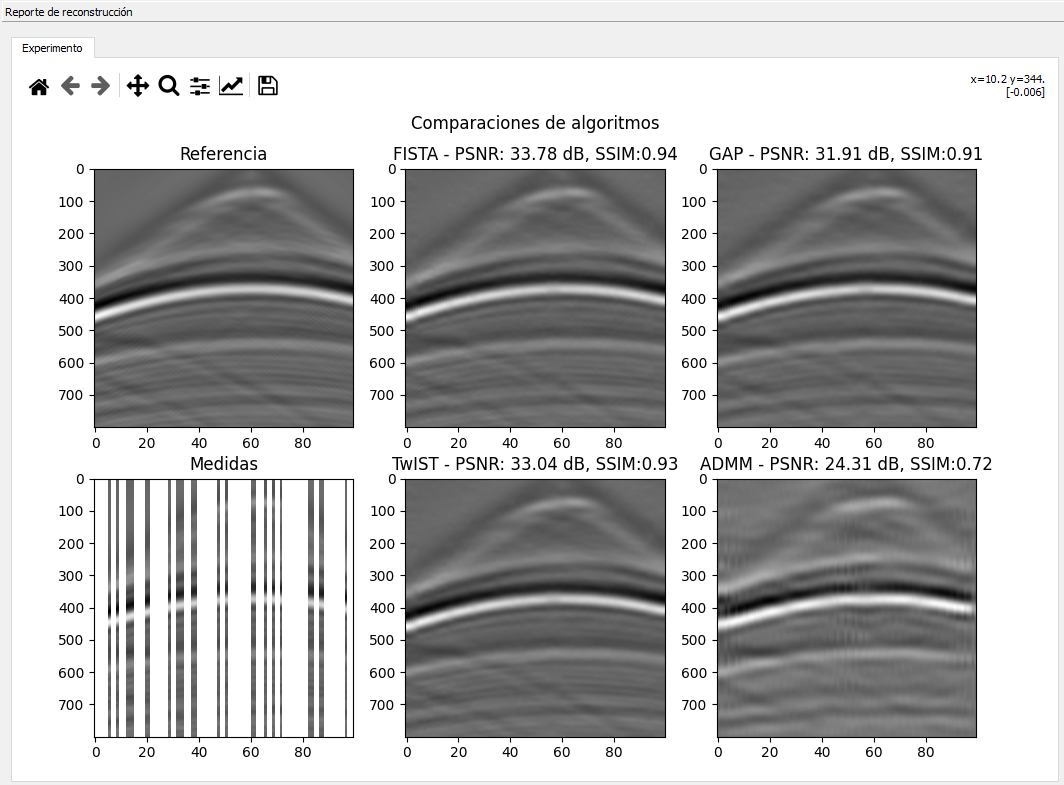
\includegraphics[width=0.9\linewidth]{result-comp2.png}
		\captionof{figure}{Reporte de reconstrucción de la comparación de algoritmos}
		\label{fig:result-comp2}
	\end{Figure}

\end{enumerate}


\section{Reconstrucción de Disparos}

Este ejemplo ilustra como realizar una reconstrucción de disparos.

\begin{enumerate}
	
	\item Inicie la aplicación ReDs y en la pantalla de inicio escoja la opción \textit{Iniciar RD}.
	
	\begin{multicols}{2}
		\item En el extremo izquierdo, en el panel \textit{Datos Sísmicos}, haga click en el botón \textit{Cargar}
		\item En la ventana \textit{Abrir dato sísmico}, como se observa en la figura \ref{fig:data_lecture_2brd}, donde el usuario podrá seleccionar un dato sísmico. Para este ejemplo cargaremos \emph{data.npy}. La aplicación ReDs reconoce las extensiones \emph{.npy} y \emph{.mat} para cargar datos sísmicos.
		\begin{Figure}
			\centering
			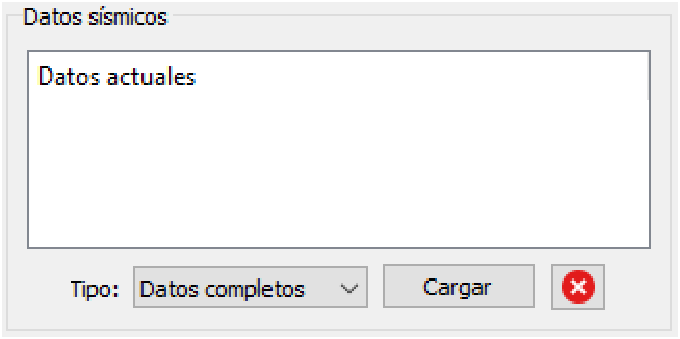
\includegraphics[width=.9\linewidth]{data-lecture-1.pdf}
			\captionof{figure}{Cargando un dato sísmico.}
			\label{fig:data_lecture_1brd}
		\end{Figure}		
	\end{multicols}
	
	\begin{Figure}
		\centering
		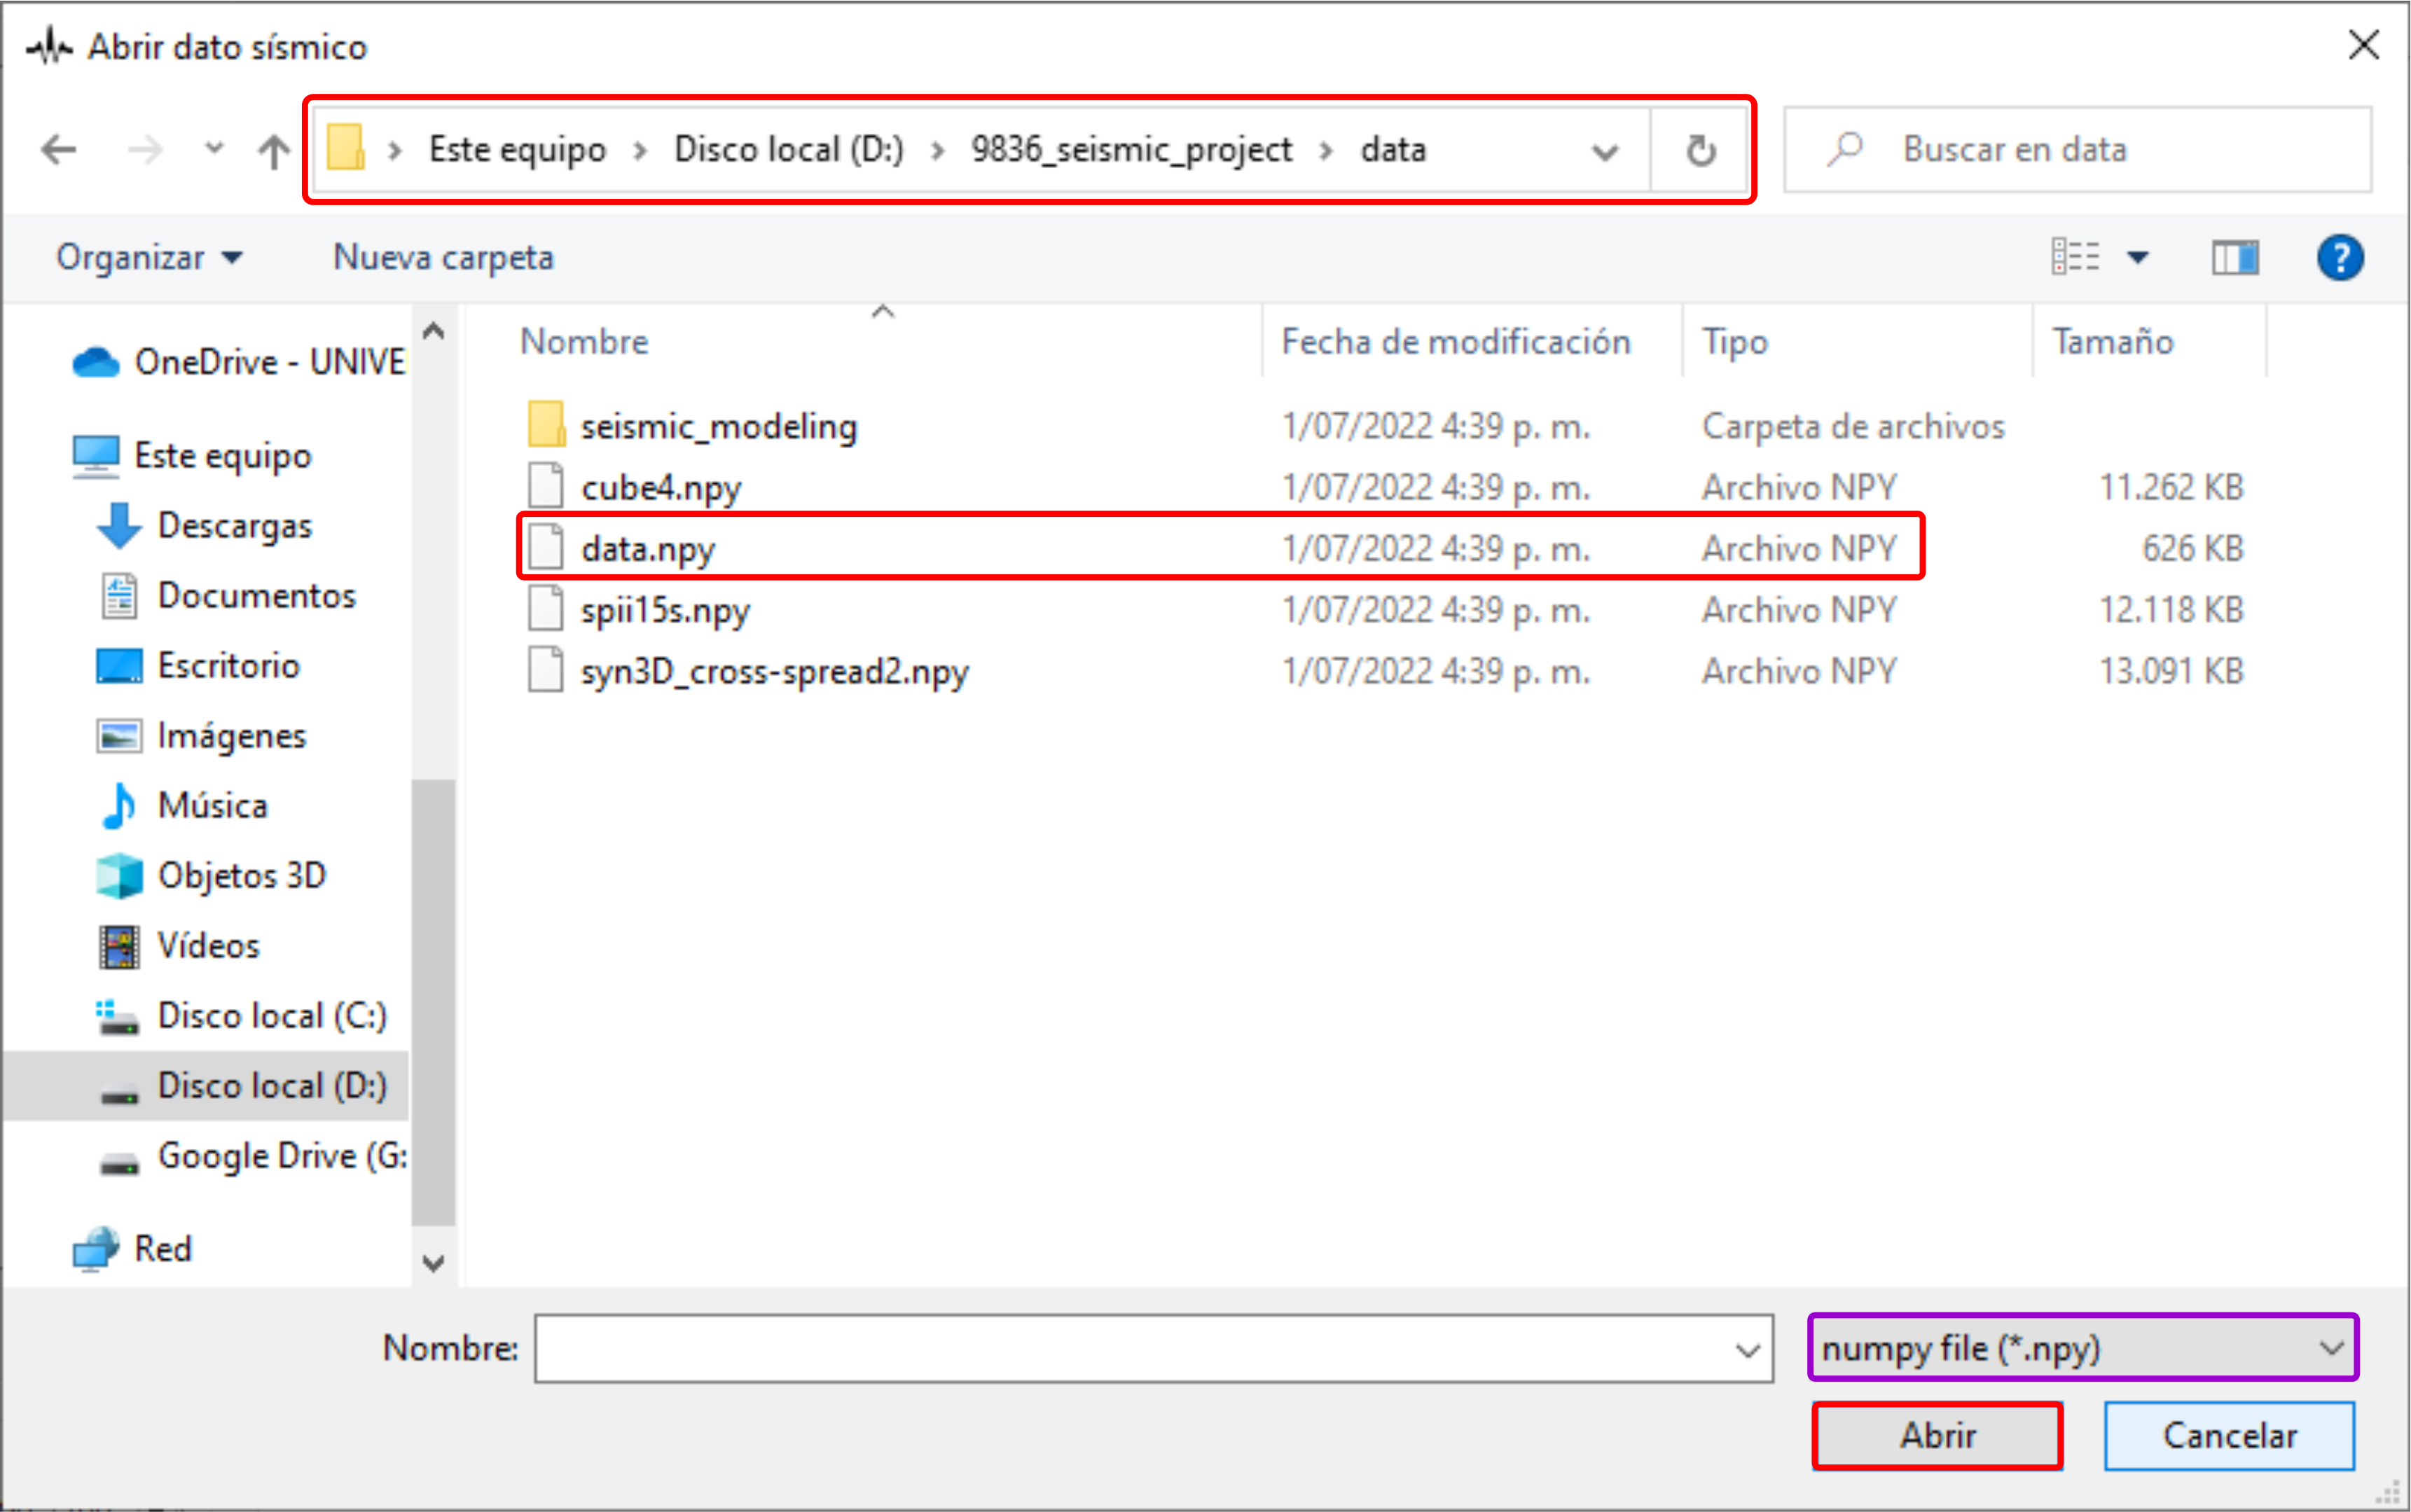
\includegraphics[width=1\linewidth]{data-lecture-2.png}
		\captionof{figure}{Ventana de selección de dato sísmico.}
		\label{fig:data_lecture_2brd}
	\end{Figure}

	\begin{multicols}{2}
		\begin{Figure}
			\vspace{5mm}
			\centering
			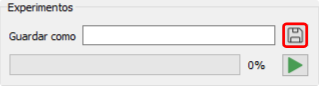
\includegraphics[width=0.9\linewidth]{experiment-1.png}
			\captionof{figure}{Panel de experimentos.}
			\label{fig:experiment_1brd}
		\end{Figure}
		\item Seleccione un archivo para guardar los resultados de la reconstrucción con el botón \hspace{0.5mm} \faSave \hspace{0.5mm} ubicado en el panel \textit{Experimentos}. En la ventana \textit{Guardar reconstrucciones} introduzca el nombre \textit{nuevo\_experimento}, tal como se observa en la figura \ref{fig:experiment_1brd}.								
	\end{multicols}

	\begin{multicols}{2}
		\item Inicie la reconstrucción pulsando el botón \hspace{0.5mm} \faPlay \hspace{0.5mm}. En la barra de progreso, a la izquierda de dicho botón, se podrá el progreso del actual experimento, como se observa en la figura \ref{fig:experiment_4brd}.		
		\begin{Figure}
			\centering
			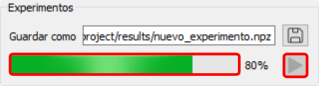
\includegraphics[width=0.7\linewidth]{experiment-4.png}
			\captionof{figure}{Ejecución de un experimento en tiempo real.}
			\label{fig:experiment_4brd}
		\end{Figure}
	\end{multicols}
	
	\item La solución de la reconstrucción de disparos se presenta en las pestañas Rendimiento y Reporte de reconstrucción, tal como se muestra en las figuras \ref{fig:result-comp1rd} y \ref{fig:result-comp2rd} respectivamente.
	
	\begin{Figure}
		\centering
		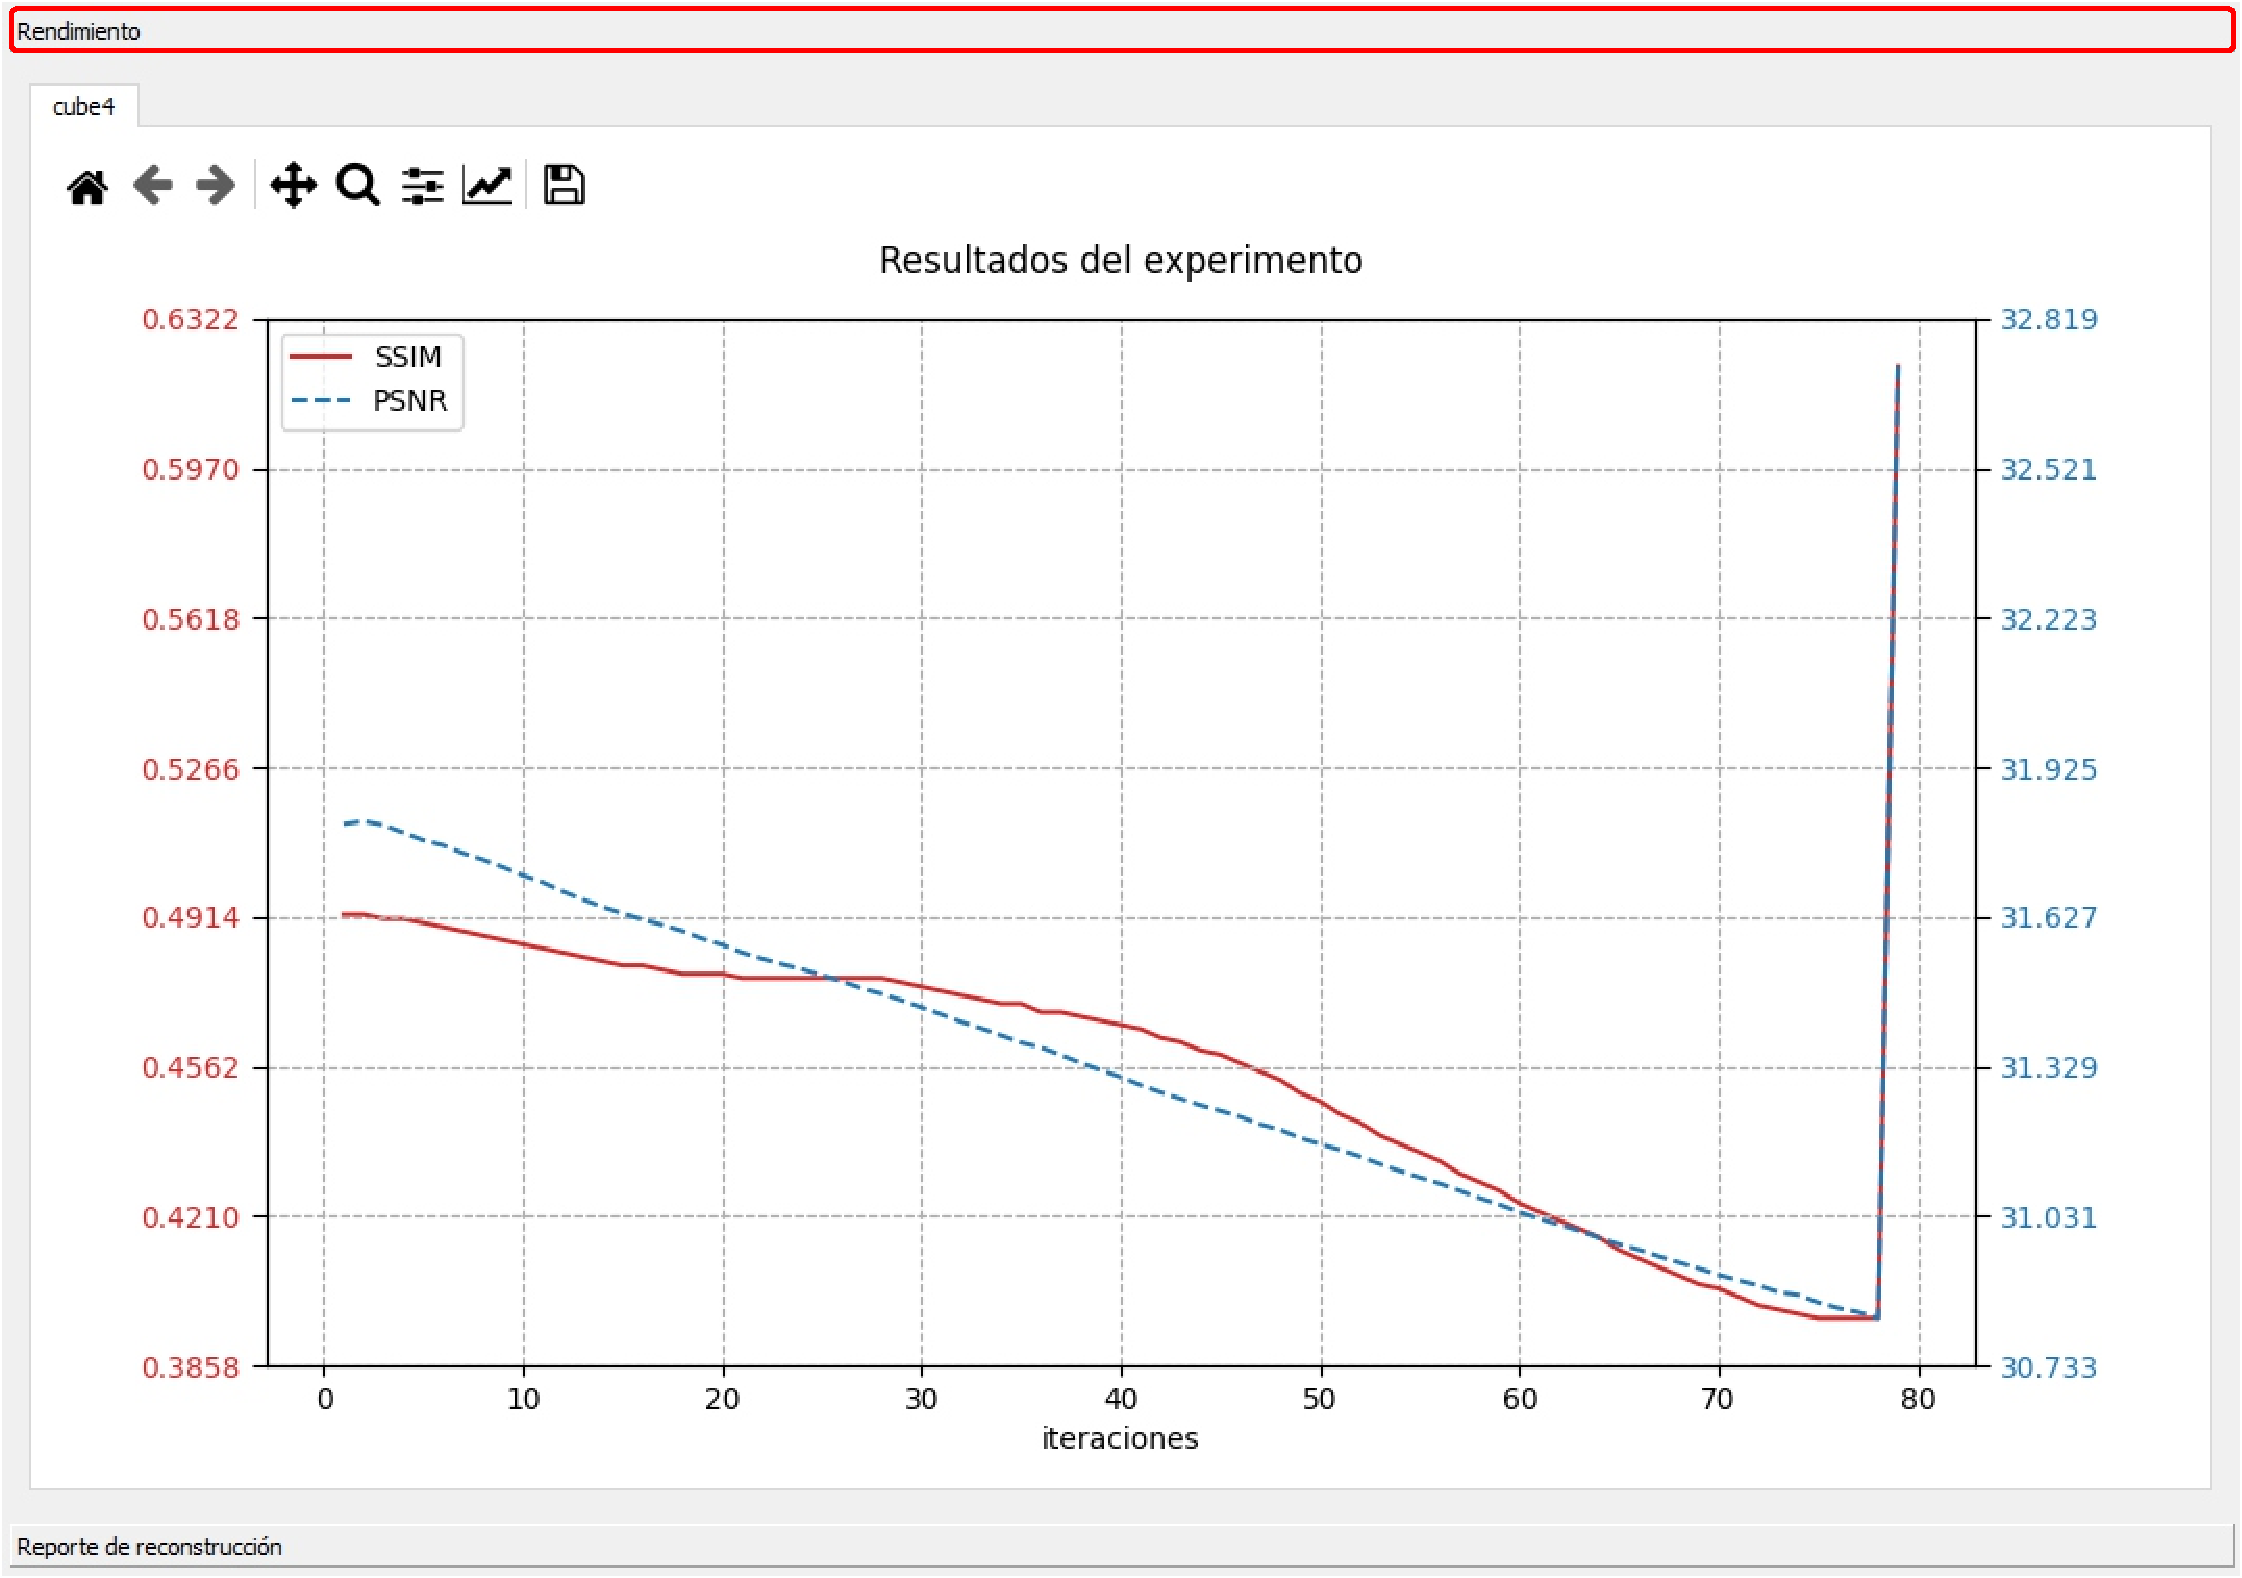
\includegraphics[width=0.75\linewidth]{rendrd}
		\captionof{figure}{Rendimiento de la reconstrucción de disparos}
		\label{fig:result-comp1rd}
	\end{Figure}
	
	\begin{Figure}
		\centering
		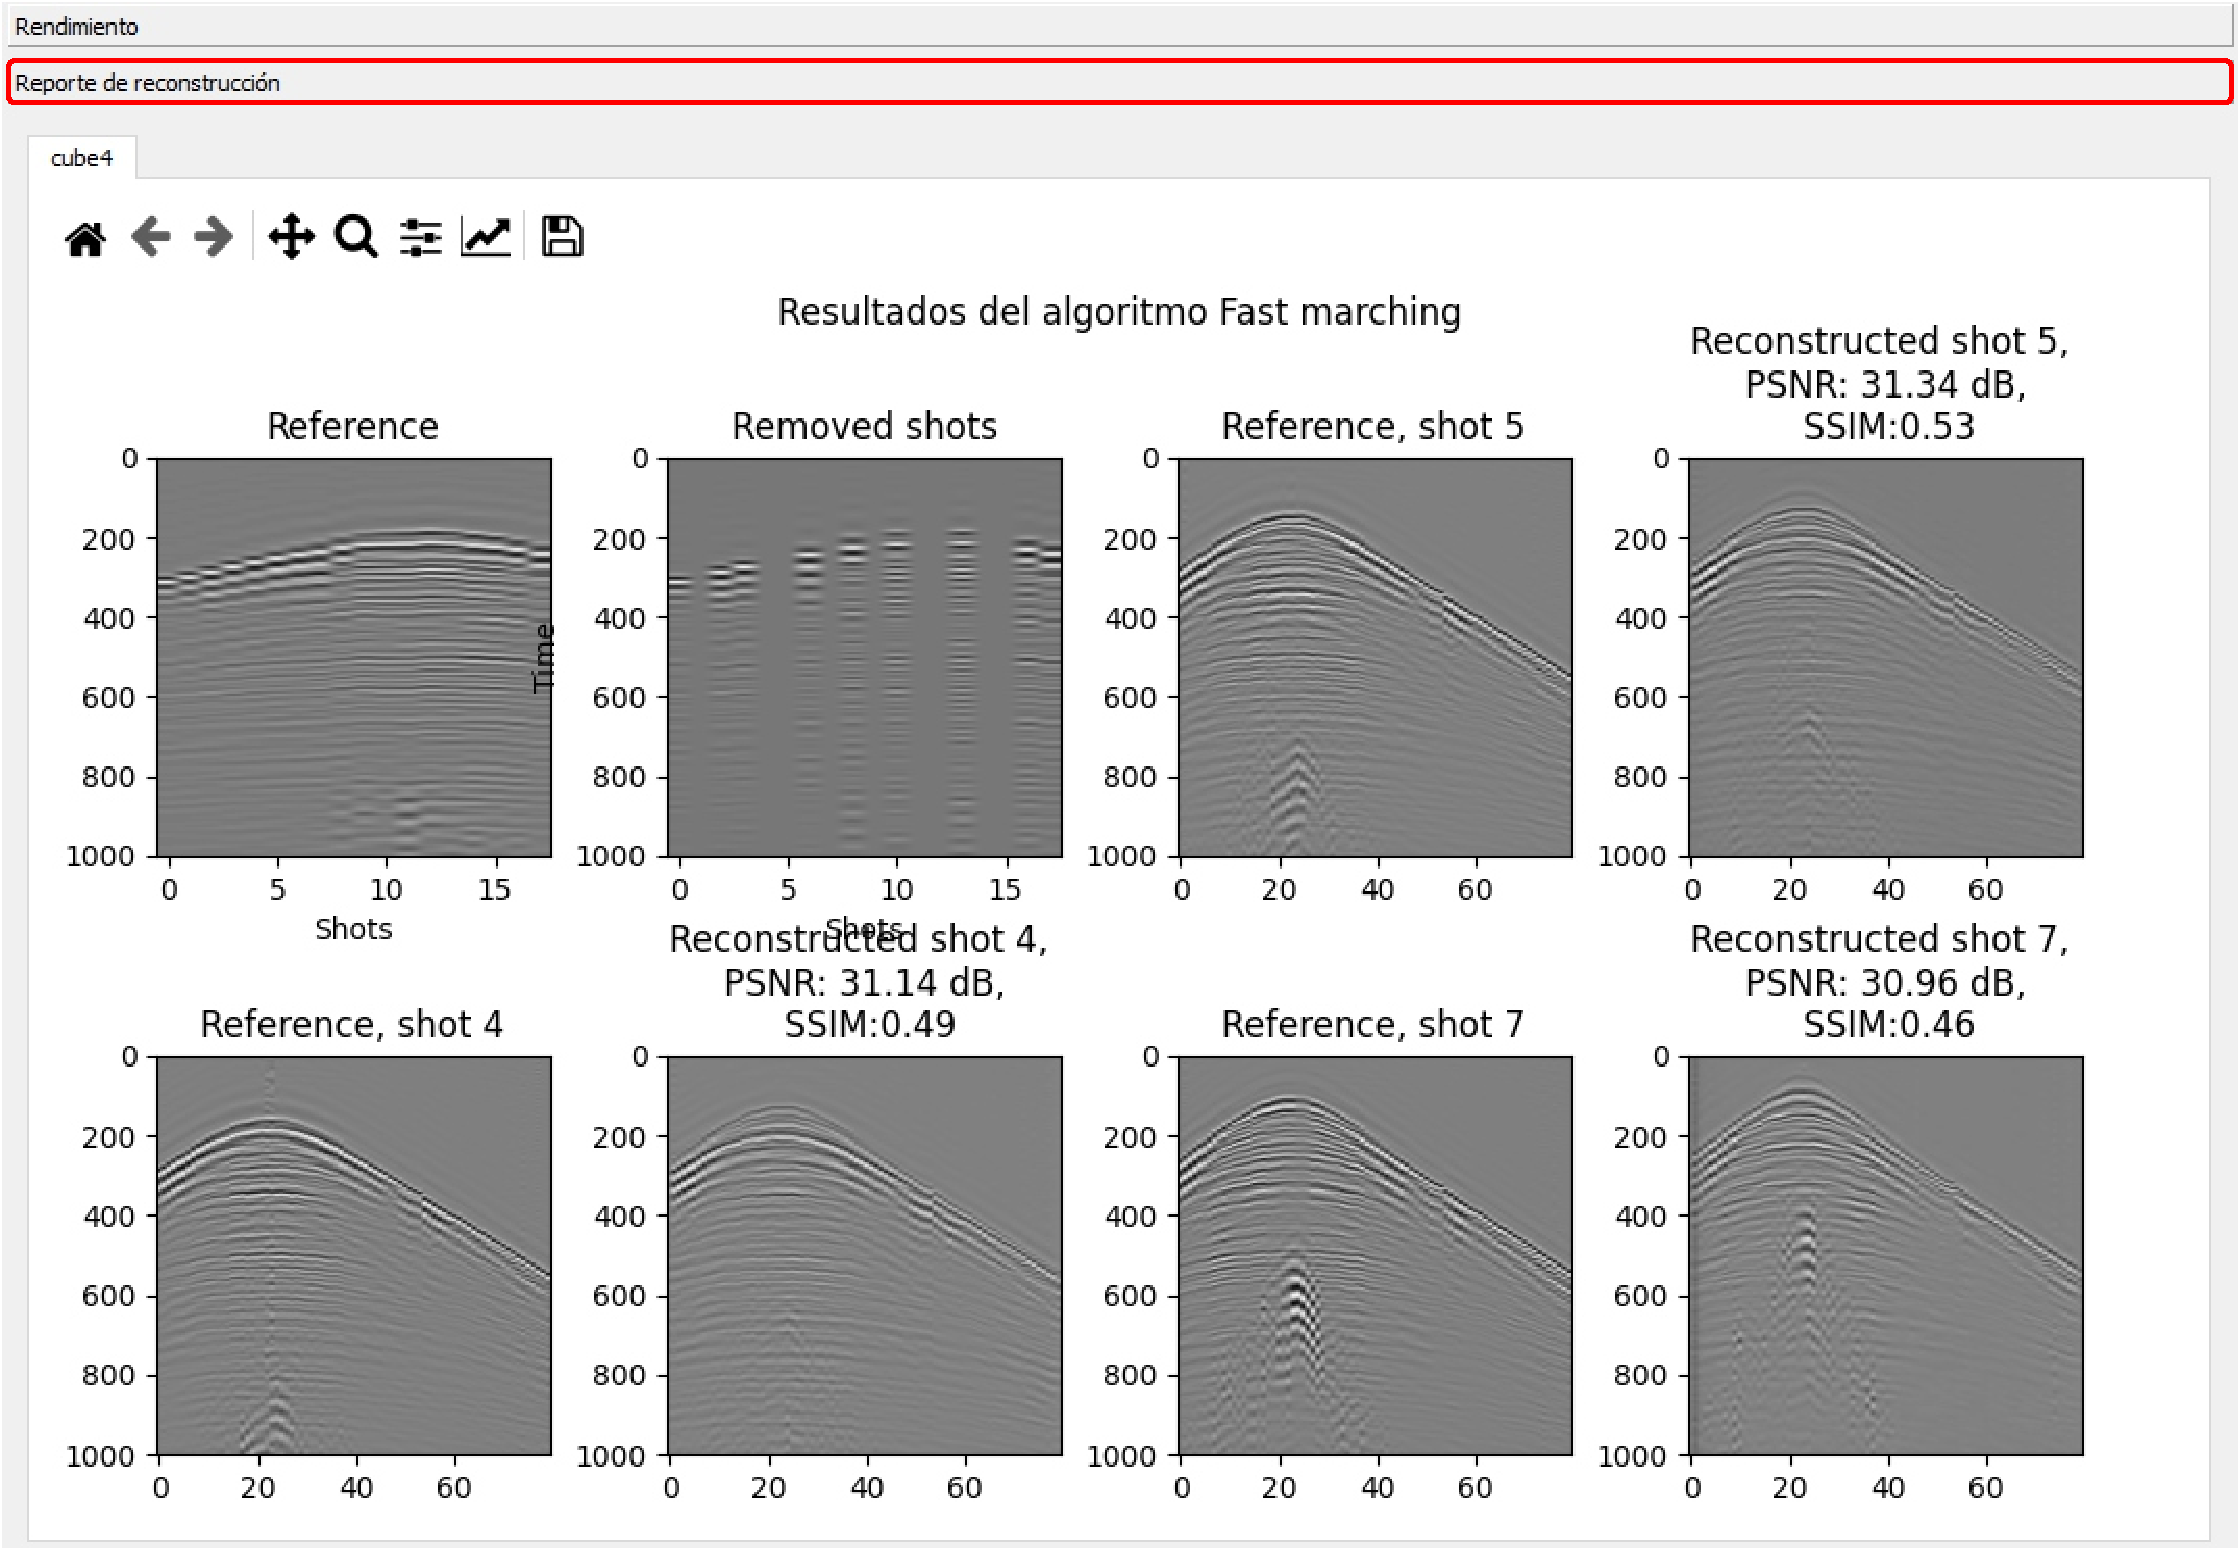
\includegraphics[width=0.75\linewidth]{rendrd2}
		\captionof{figure}{Reporte de la reconstrucción de disparos}
		\label{fig:result-comp2rd}
	\end{Figure}
	
\end{enumerate}	

\end{document}